% Author: Seongjin Lee 
% Gyeongsang National University, Korea 
% 
% 2017-03-06
%

\documentclass[newPxFont,sthlmFooter,nooffset]{beamer}
\usepackage{kotex}
%\usetheme{sthlm}
\usepackage{../style/beamerthemesthlm}
\hypersetup{pdfauthor={Seongjin Lee (insight@gnu.ac.kr)},
            pdfsubject={Data Structure and Algorithm, Lecture Note},
            pdfkeywords={Data Structure, Algorithm, Lecture, Note},
            pdfmoddate={D: \pdfdate},
            pdfcreator={Seongjin Lee}}

%\setbeamertemplate{footline}[text line]{%
%    \parbox{\linewidth}{\vspace*{-8pt} \insertsectionhead  \hfill\insertshortauthor\hfill\insertpagenumber}}
%\setbeamertemplate{navigation symbols}{}


\setbeamertemplate{blocks}[rounded]

\title{Data Structure and Algorithm}
\subtitle{Class 7}
\author[SJL]{Seongjin Lee}
\institute{\href{mailto:insight@gnu.ac.kr}{insight@gnu.ac.kr}\\\url{http://resourceful.github.io}\\Systems Research Lab.\\GNU}
\date{2017-03-06} 

\begin{document}



\frame[plain,t]{\titlepage} 

\frame{\frametitle{Table of contents}\tableofcontents} 


%---------------------------------------------------------

\section{Tree} 
\begin{frame}[t]
  \frametitle{Introduction}
  \begin{description}
  \item[\textbf{Tree}] It is finite set of one or more nodes such that
    \begin{enumerate}
      \item there is a special node called root
      \item remaining nodes are partitioned into n$geq$0 disjoint trees $T_1$, $T_2$, $\cdots$, $T_n$ where each of these is a tree; we call each $T_i$ subtree of the root
    \end{enumerate}
  \item[\textbf{Acyclic graph}] A tree that contains no cycle
  \end{description}

It has a hierarchical structure
\end{frame}

\begin{frame}[t]
  \frametitle{Tree}
  \begin{center}
    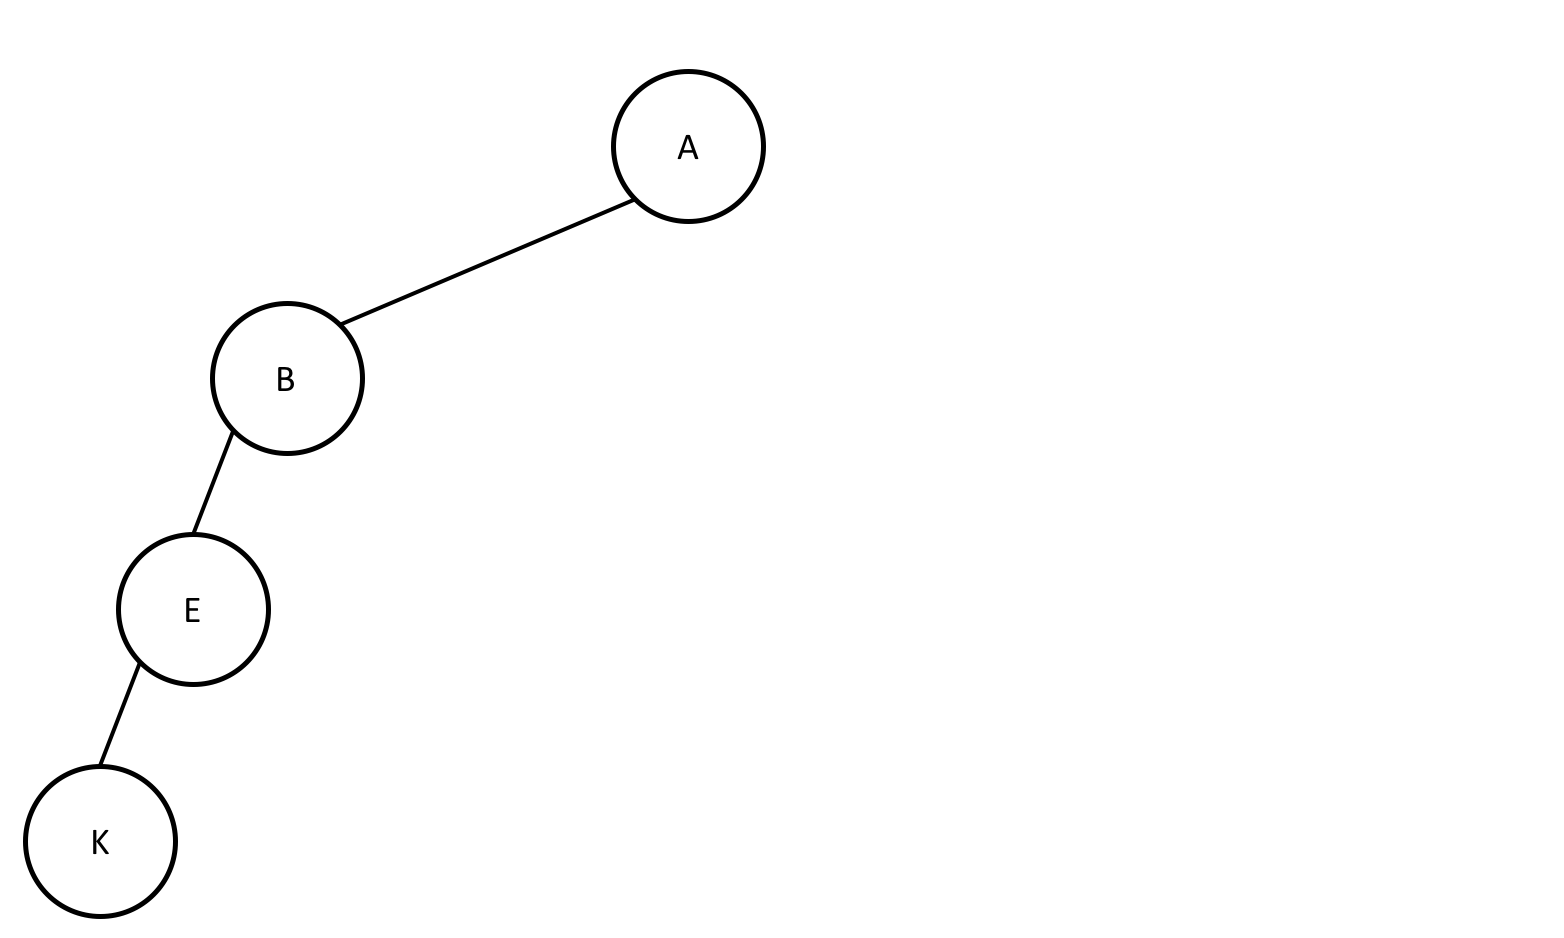
\includegraphics[width=0.8\textwidth]{figures/fig01_tree1.png}
  \end{center}

\end{frame}

\begin{frame}[t]
  \frametitle{Tree}
  \begin{center}
    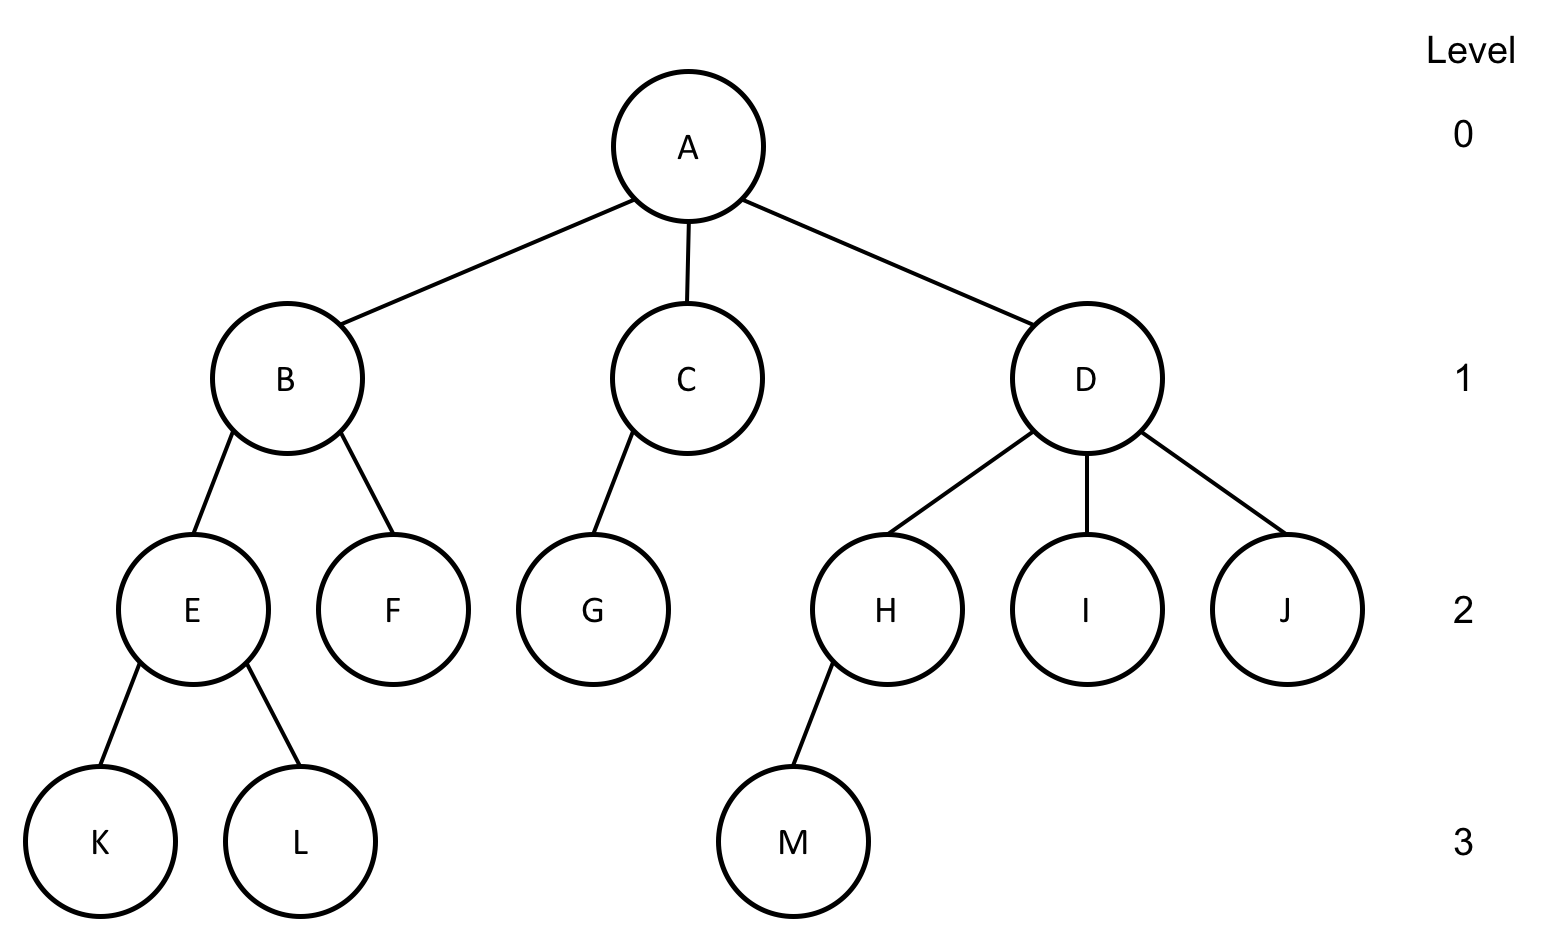
\includegraphics[width=0.8\textwidth]{figures/fig01_tree2.png}
  \end{center}

\end{frame}

\section{Terminology}

\begin{frame}[t, allowframebreaks]
  \frametitle{Terminology}
  \begin{description}
  \item[\textbf{Root}] A node with no parent (e.g., A is the root)\\
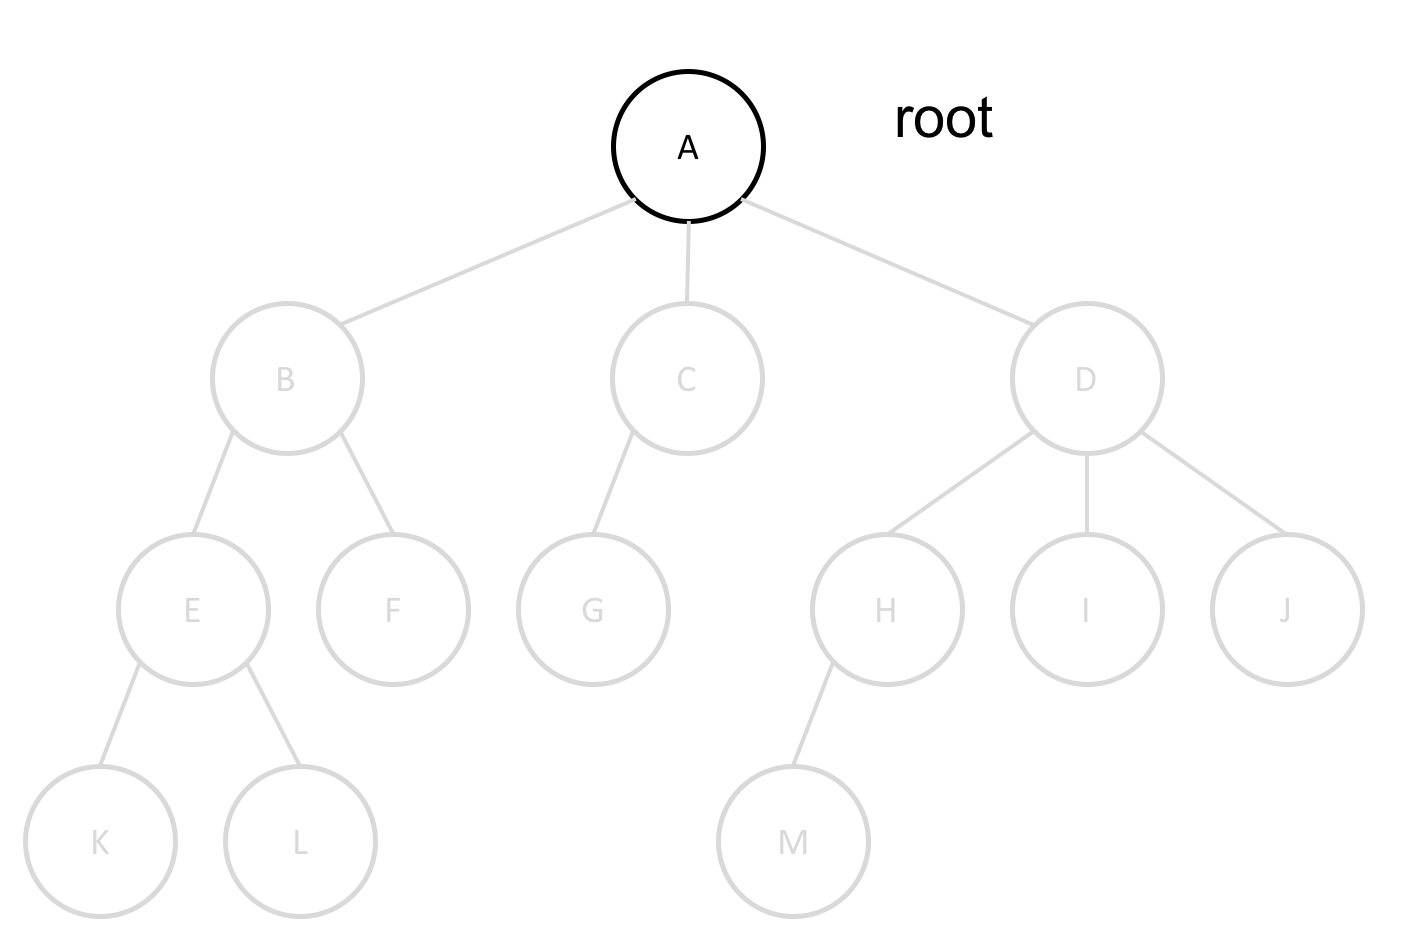
\includegraphics[height=0.3\textheight]{./figures/fig02_def_root.png}
  \item[\textbf{edge}] The connecting link between any two nodes (e.g., link between A and B is edge)\\
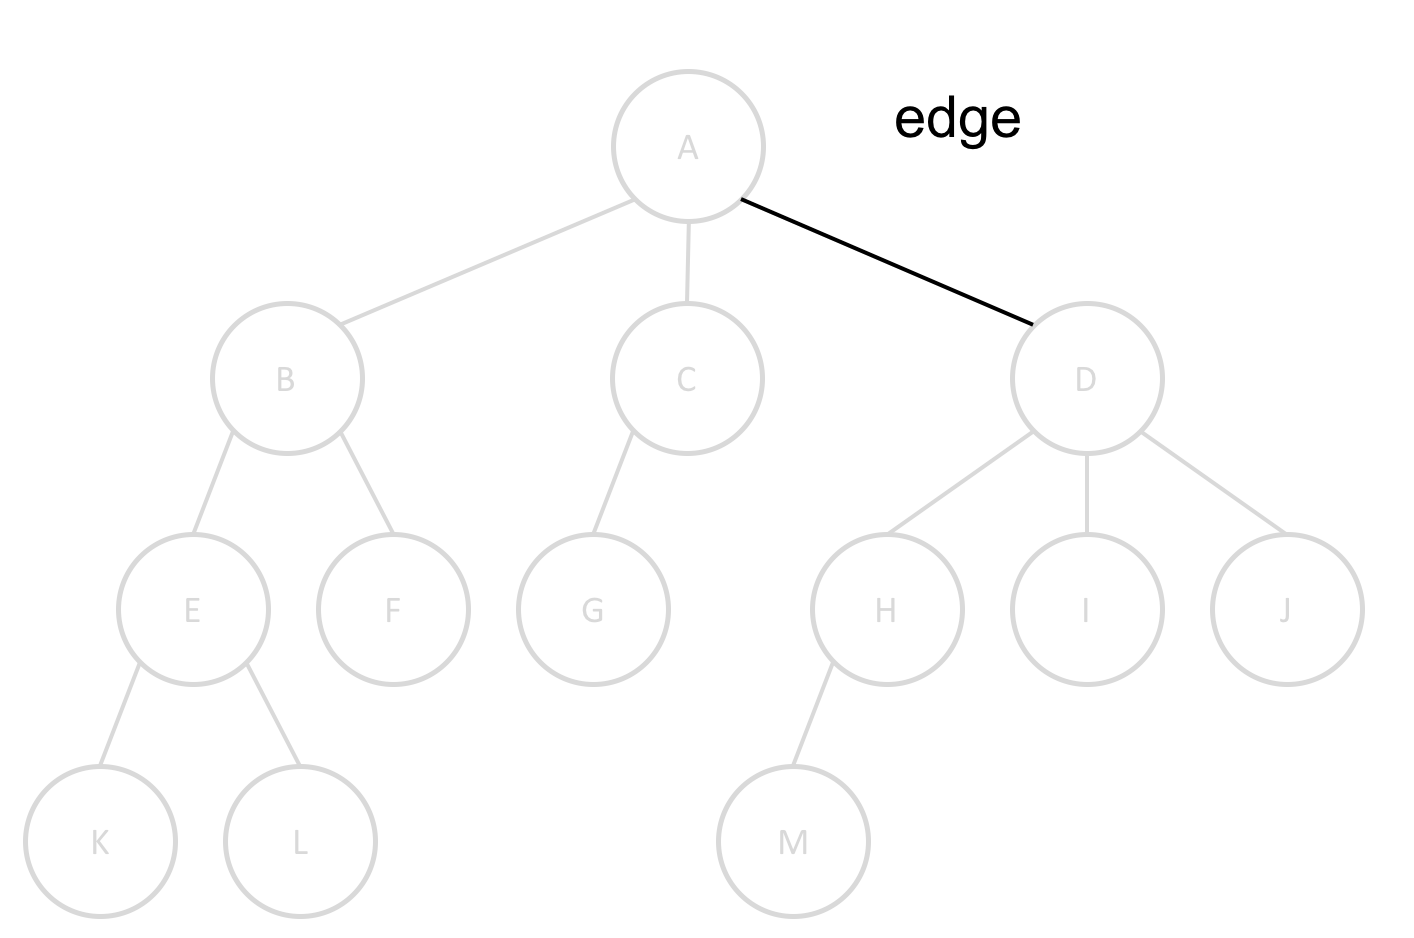
\includegraphics[height=0.3\textheight]{./figures/fig02_def_edge.png}
  \item[\textbf{parent}] a node that has subtrees (e.g., A is parent of B, C, and D. E is parent of K and L)\\
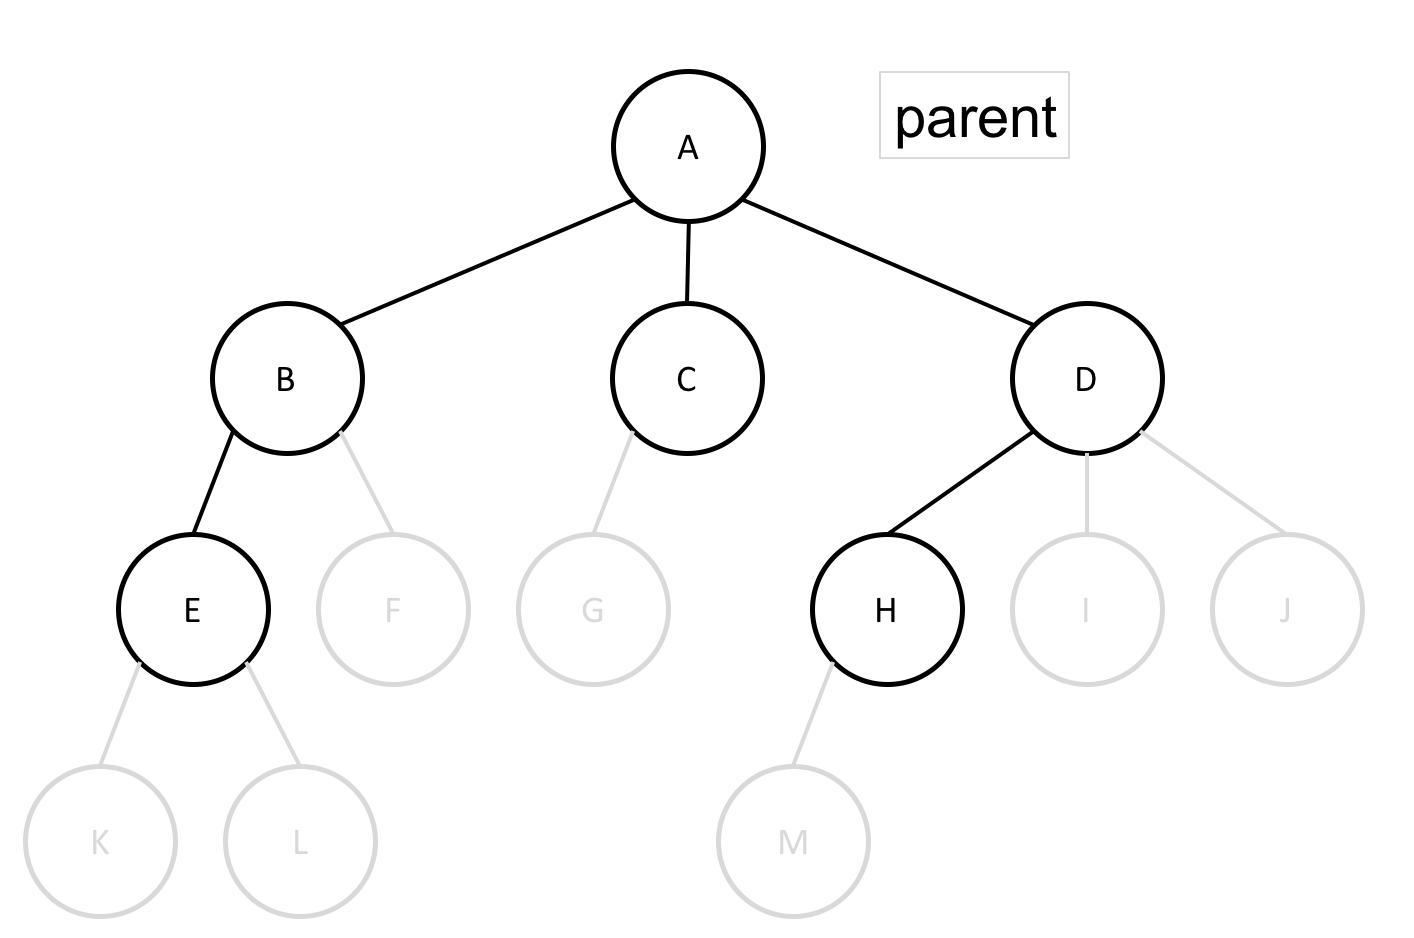
\includegraphics[height=0.3\textheight]{./figures/fig02_def_parent.png}
  \item[\textbf{child}] a root of the subtrees (e.g., E is child of B, C is child of A)\\
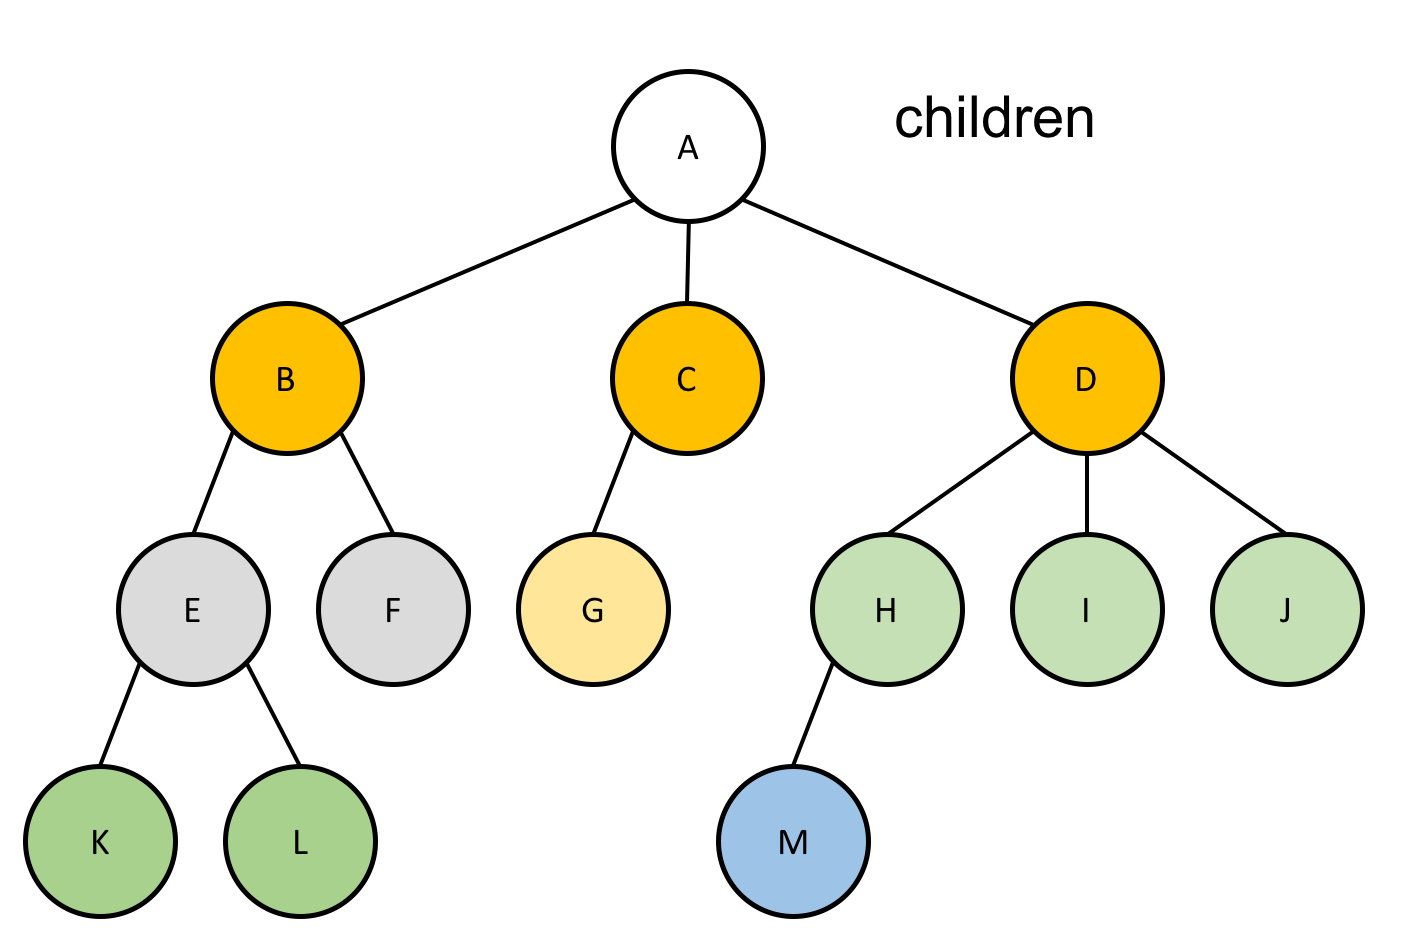
\includegraphics[height=0.3\textheight]{./figures/fig02_def_children.png}
  \item[\textbf{sibling}] child nodes of the same parent (e.g., B, C, and D are siblings, K, L, and M are siblings)\\
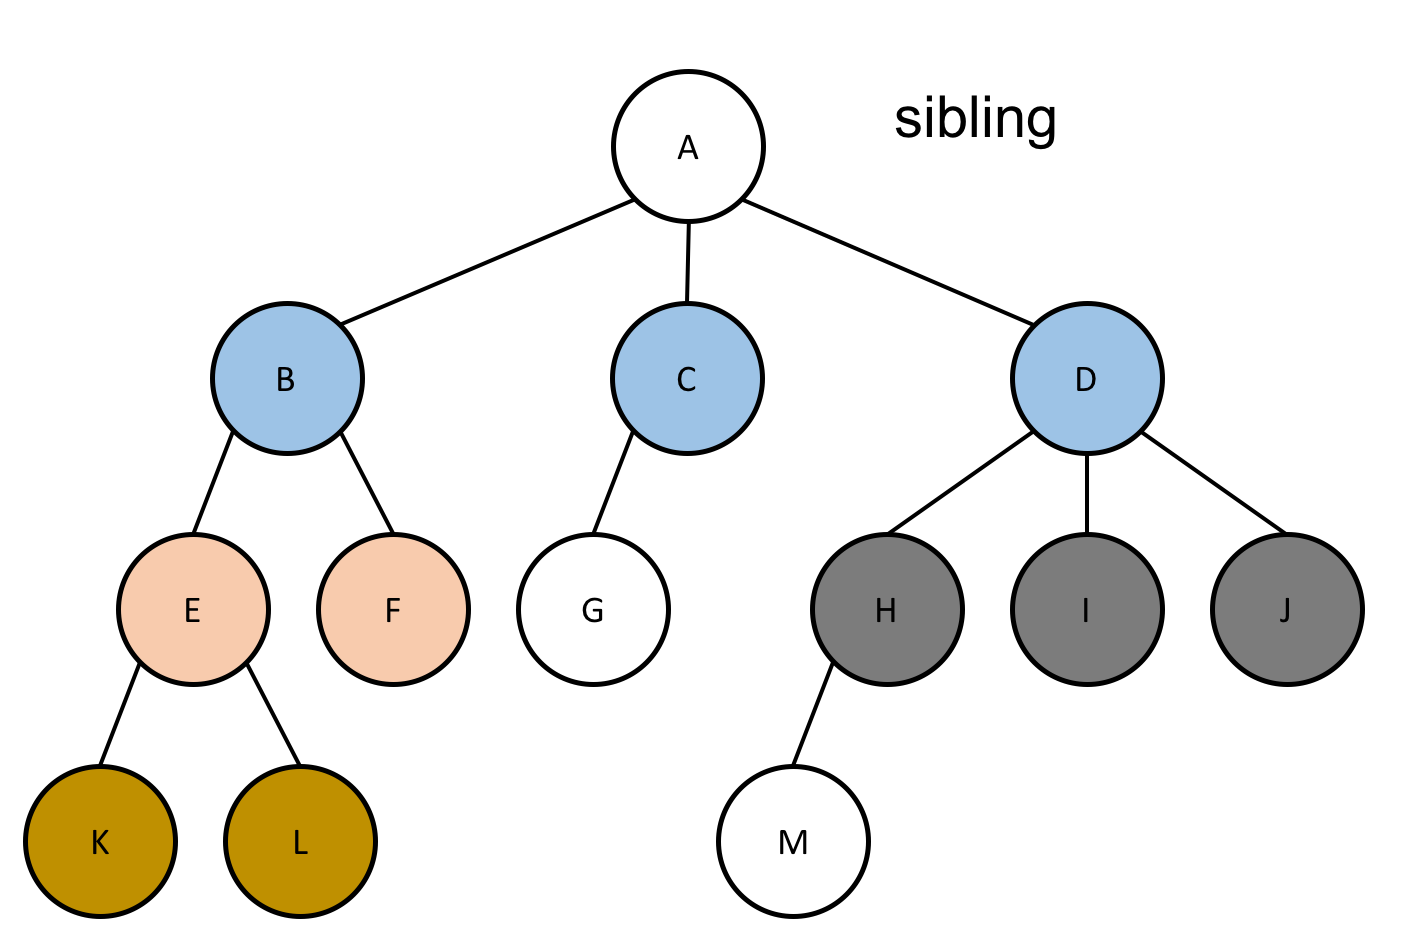
\includegraphics[height=0.3\textheight]{./figures/fig02_def_sibling.png}
  \item[\textbf{Leaf (terminal, external) node}] A node with degree
    zero (e.g., K, L, F, G, M, I, and J)\\
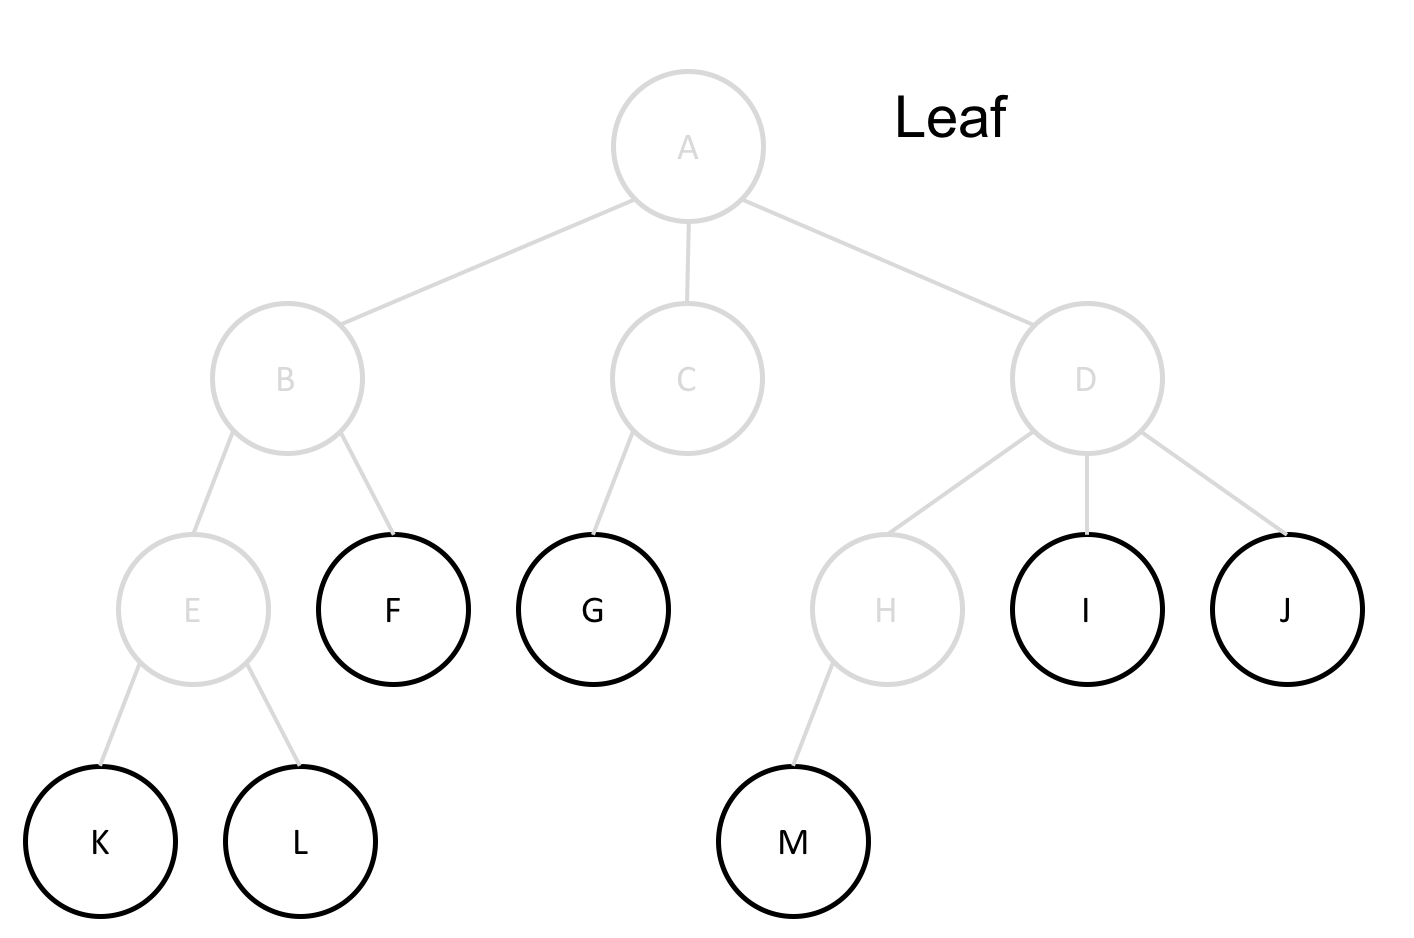
\includegraphics[height=0.3\textheight]{./figures/fig02_def_leaf.png}
  \item[\textbf{Internal (non-terminal, internal) node}] node with
    degree one or more (e.g., A, B, C, D, E, and H)
  \item[\textbf{ancestor}] all the nodes along the path from the root
    to the node (e.g., ancestor of K is K, E, B, and A. Ancestor of H
    is H, D, and A)\\
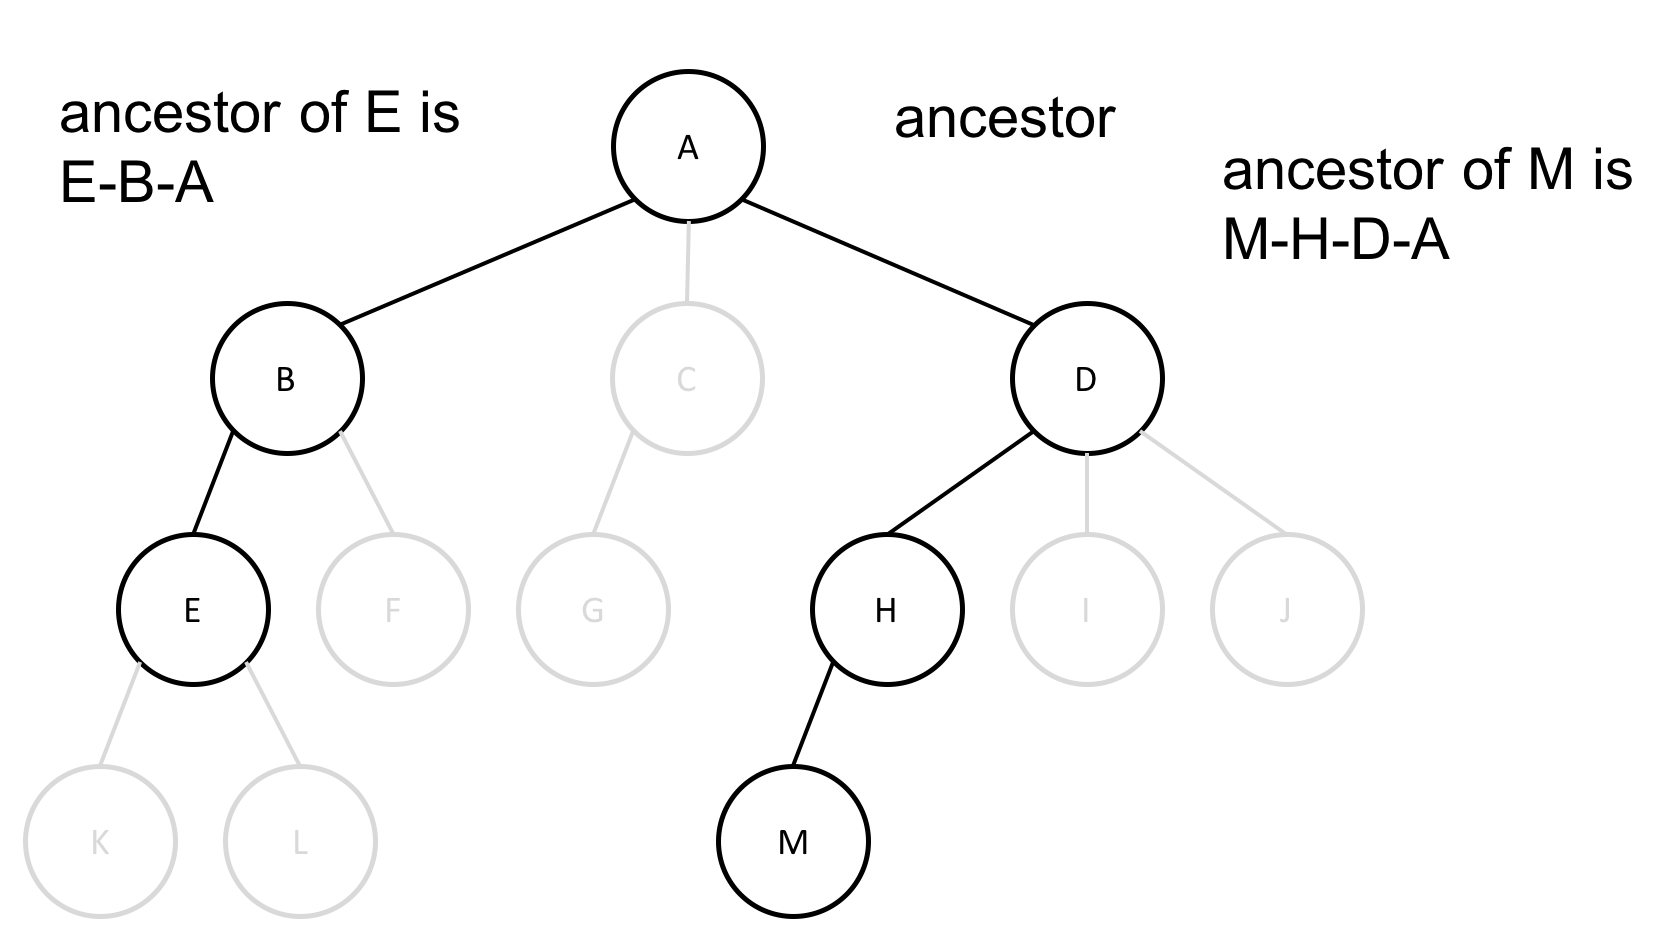
\includegraphics[height=0.3\textheight]{./figures/fig02_def_ancestor.png}
  \item[\textbf{descendant}] all the nodes that are in its subtrees
    (e.g., Descendants of E is E, K, and L. Descendants of D is D, H,
    M, I, and J)\\
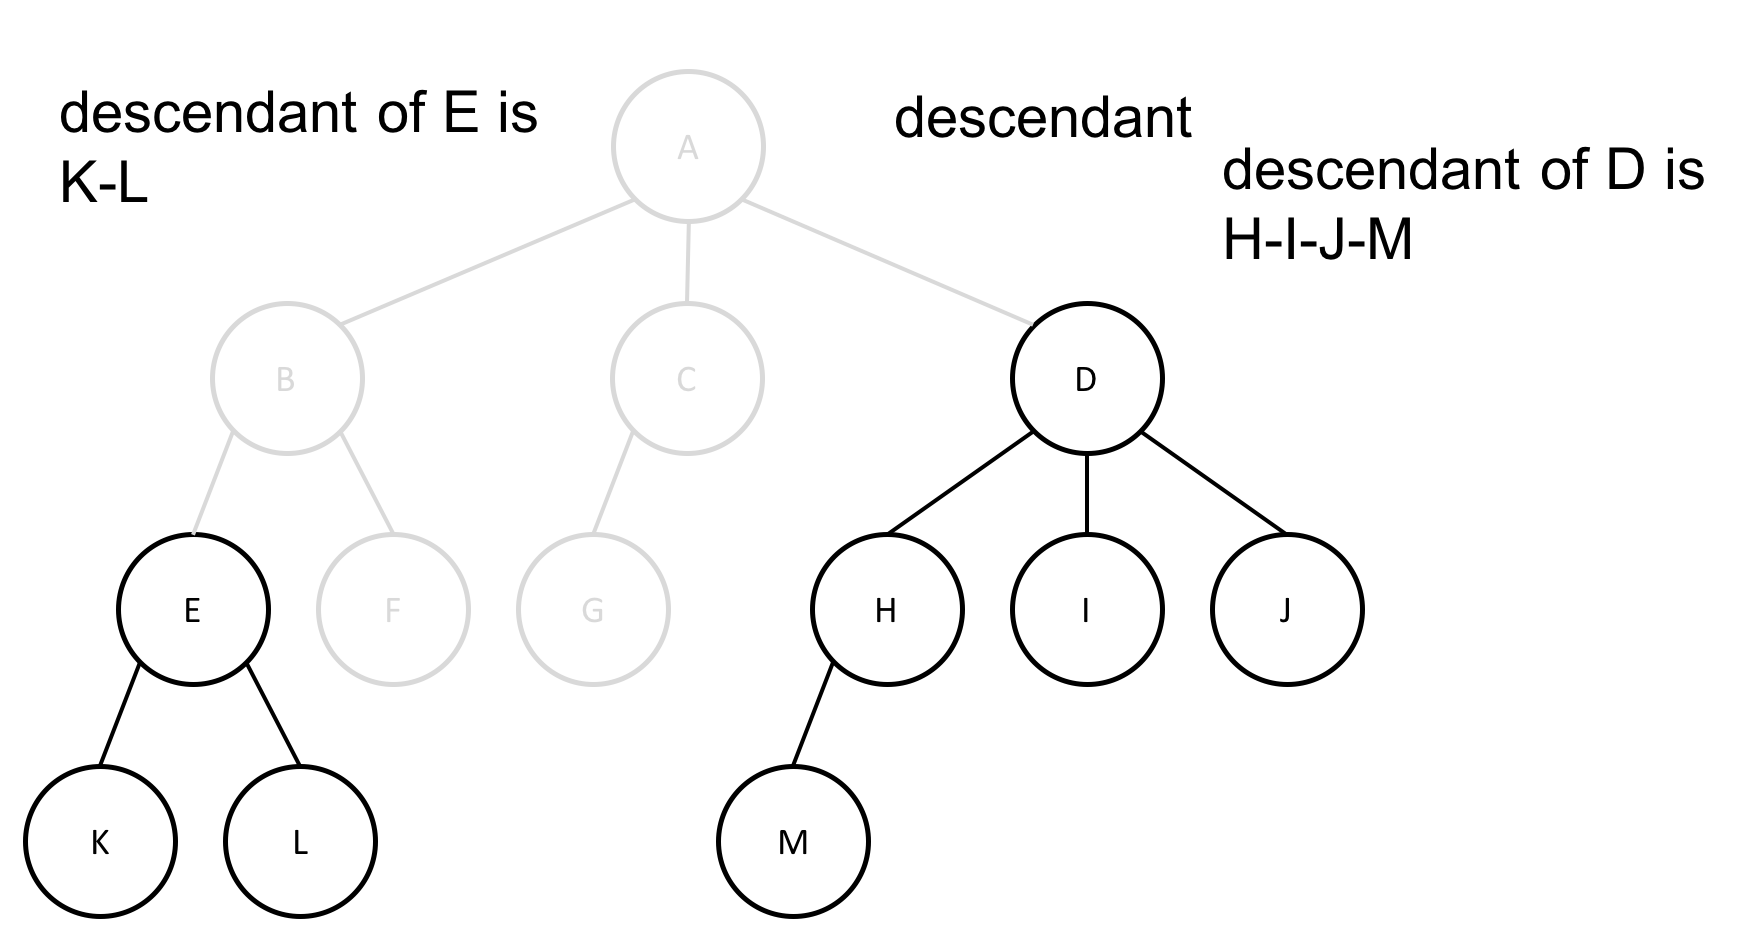
\includegraphics[height=0.3\textheight]{./figures/fig02_def_descendant.png}
  \item[\textbf{Degree of a node}] The number of subtrees of node, in
    other words the total number of children of a node (e.g., Degree
    of A is 3. Degree of C is 1)
  \item[\textbf{Degree of a tree}] The maximum degree of the nodes in
    the tree (e.g., the degree of the tree is 3)\\
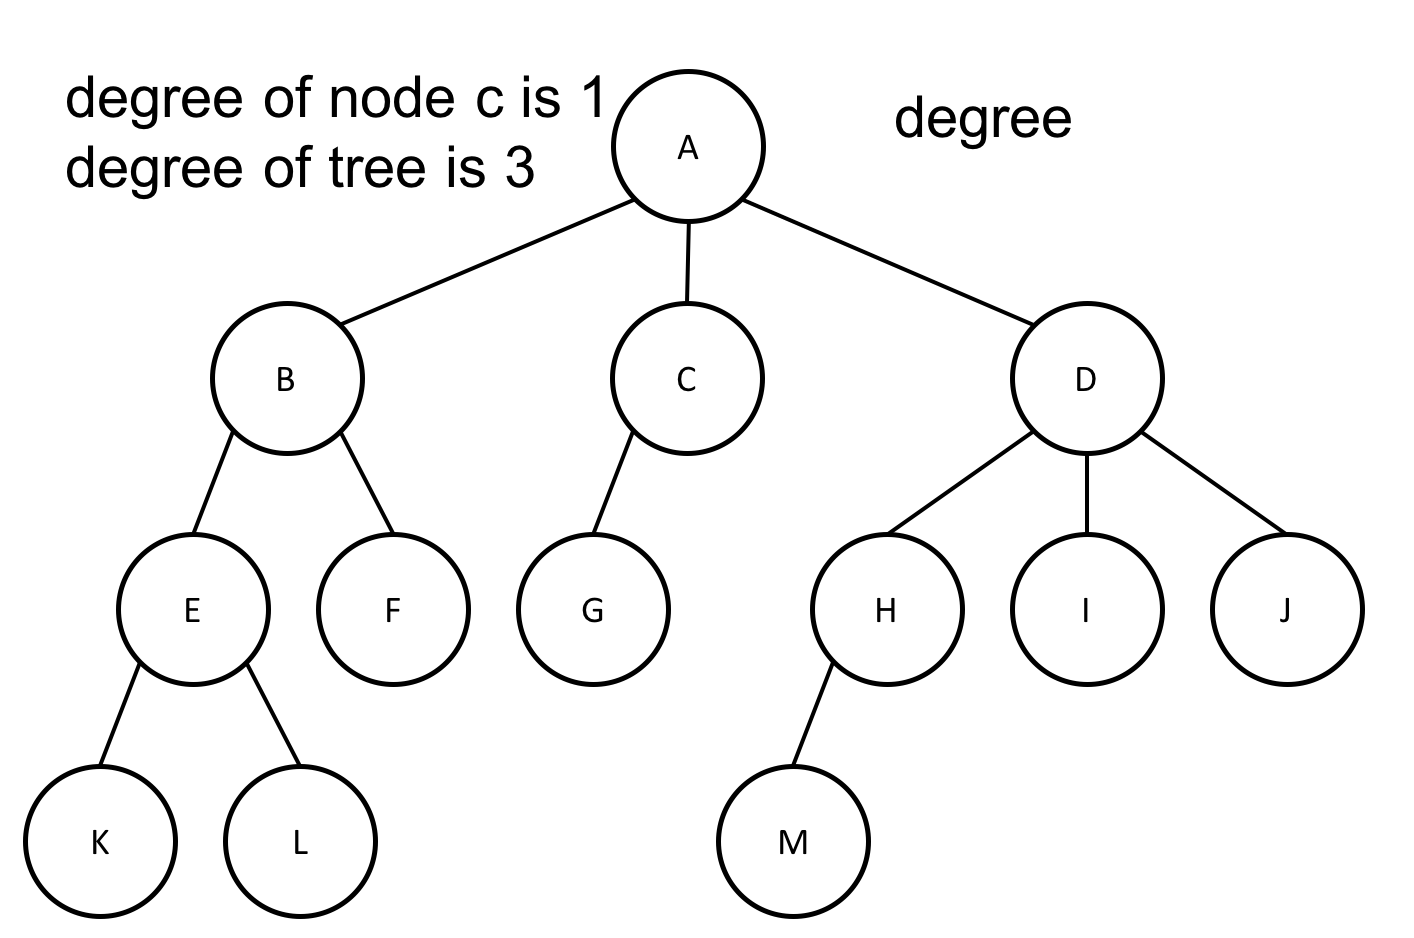
\includegraphics[height=0.3\textheight]{./figures/fig02_def_degree.png}
  \item[\textbf{level}] each step from top to bottom, the level of the
    root node is 0 (e.g., level of F is 2. Level of M is 3)\\
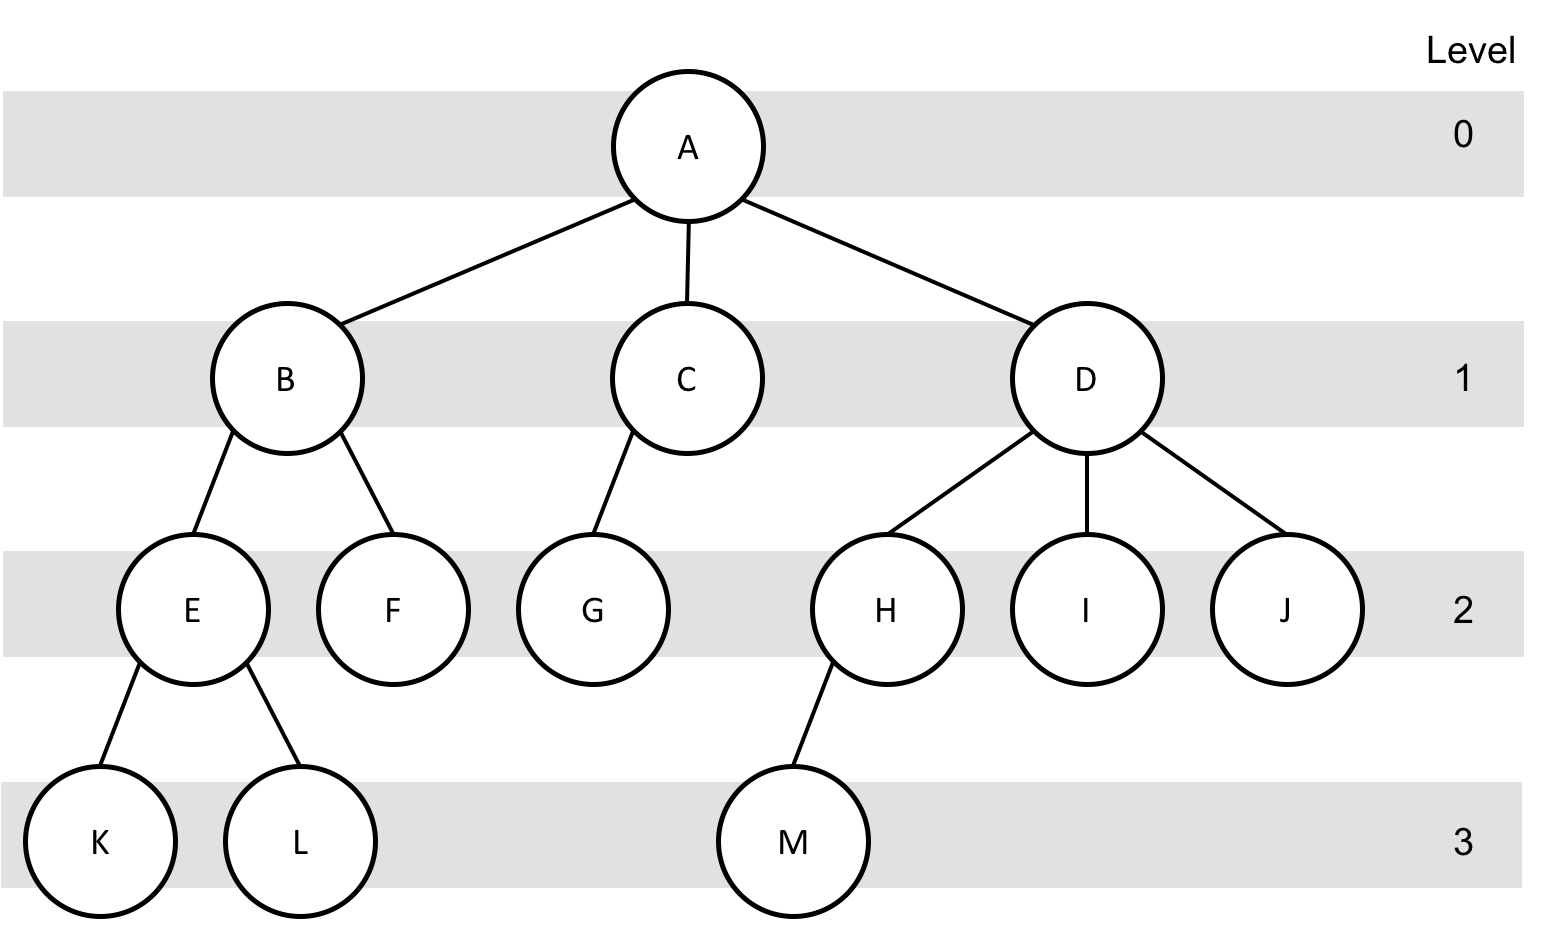
\includegraphics[height=0.3\textheight]{./figures/fig02_def_level.png}
  \item[\textbf{path}] the set of edges from the root to a node (e.g.,
    the path to M from A is (A, D), (D, H), (H, M))
  \item[\textbf{path length}] The number of edges in a path (e.g.,
    path length from A to M is 3)\\
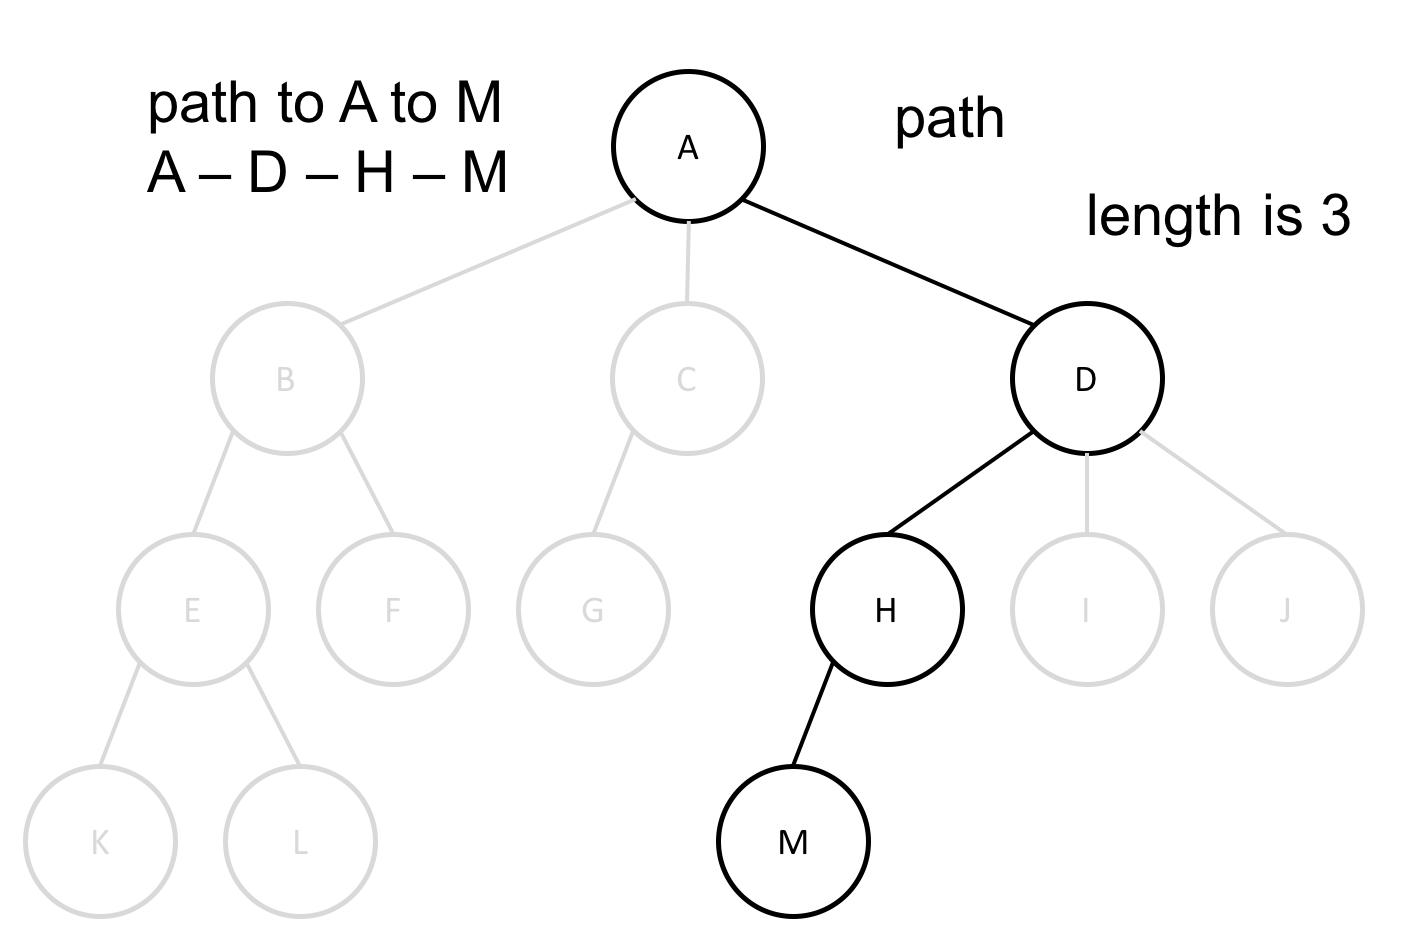
\includegraphics[height=0.3\textheight]{./figures/fig02_def_path.png}
  \item[\textbf{Height of a tree}] The longest path length from the
    root to a leaf (e.g., the height is 3)\\
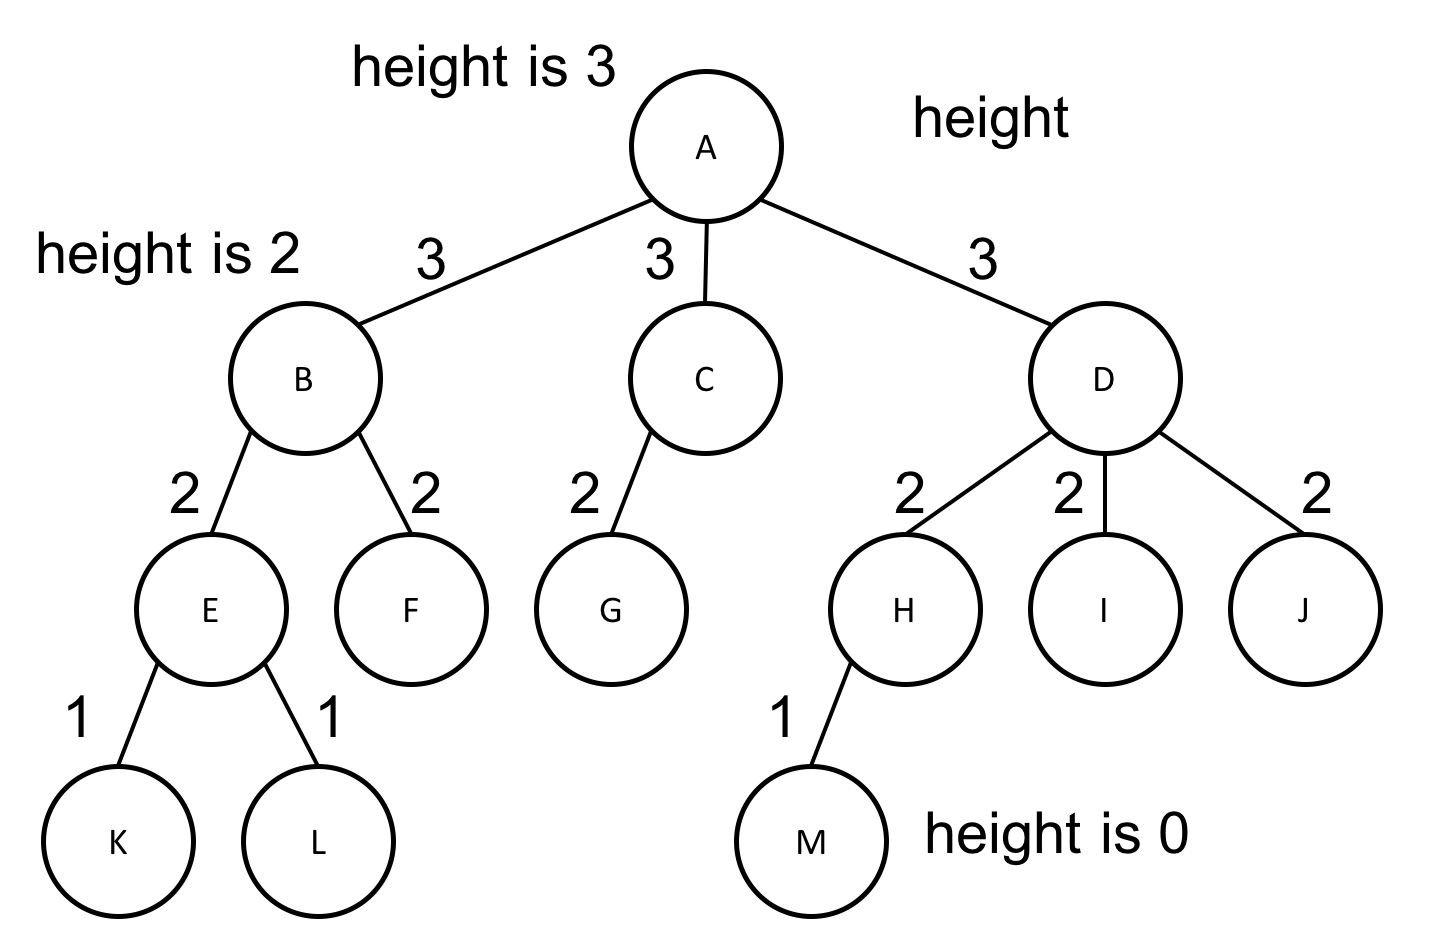
\includegraphics[height=0.3\textheight]{./figures/fig02_def_height.png}
\newpage  \item[\textbf{depth}] the total number of edges from root node to a
    particular node (e.g., depth of F is 2. Depth of M is 3)
  \item[\textbf{depth of the tree}] the total number of edges from
    root node to a leaf node in the longest path (e.g., depth of the
    tree is 3)\\
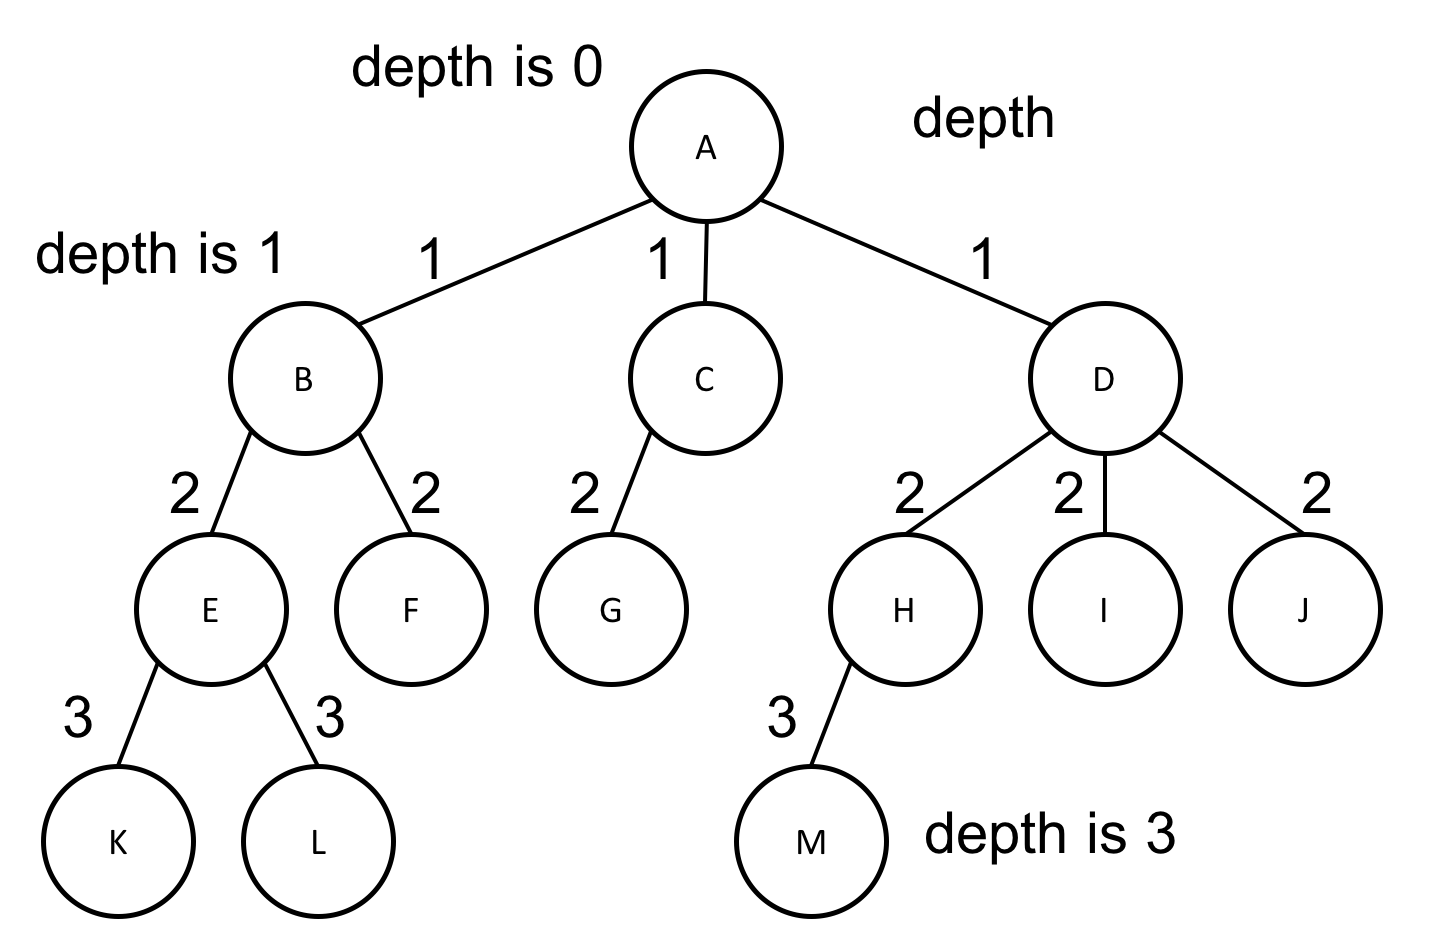
\includegraphics[height=0.3\textheight]{./figures/fig02_def_depth.png}
  \item[\textbf{subtree}] each child from a node forms a subtree
    recursively. Every child node will form a subtree on its parent
    node\\
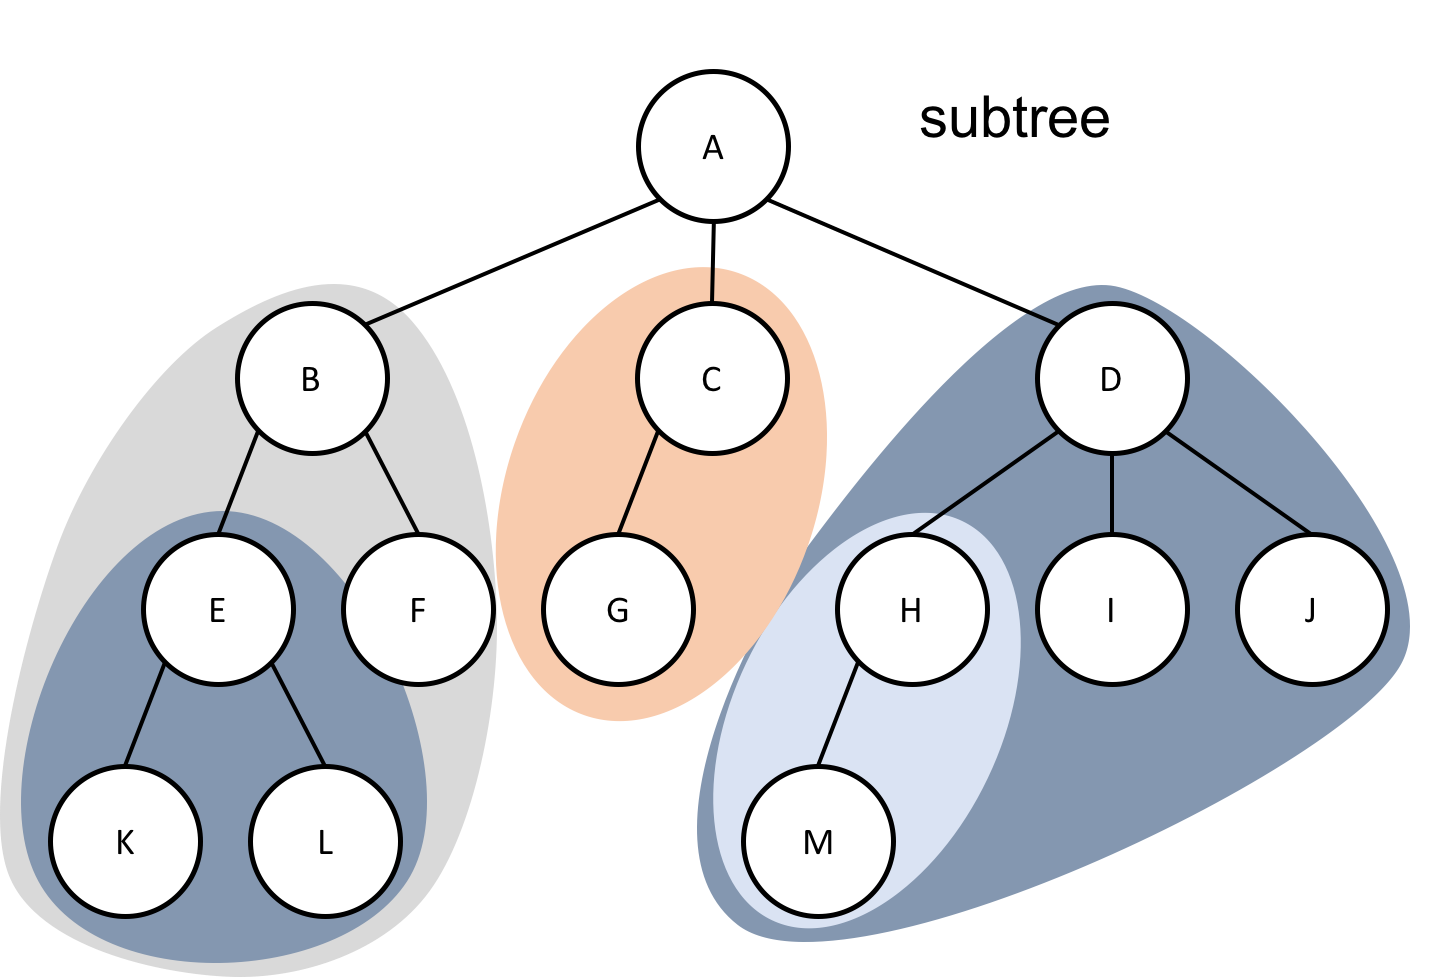
\includegraphics[height=0.3\textheight]{./figures/fig02_def_subtree.png}
\item[\textbf{proper (or full) tree}] every node other than the leaves has non-void children\\
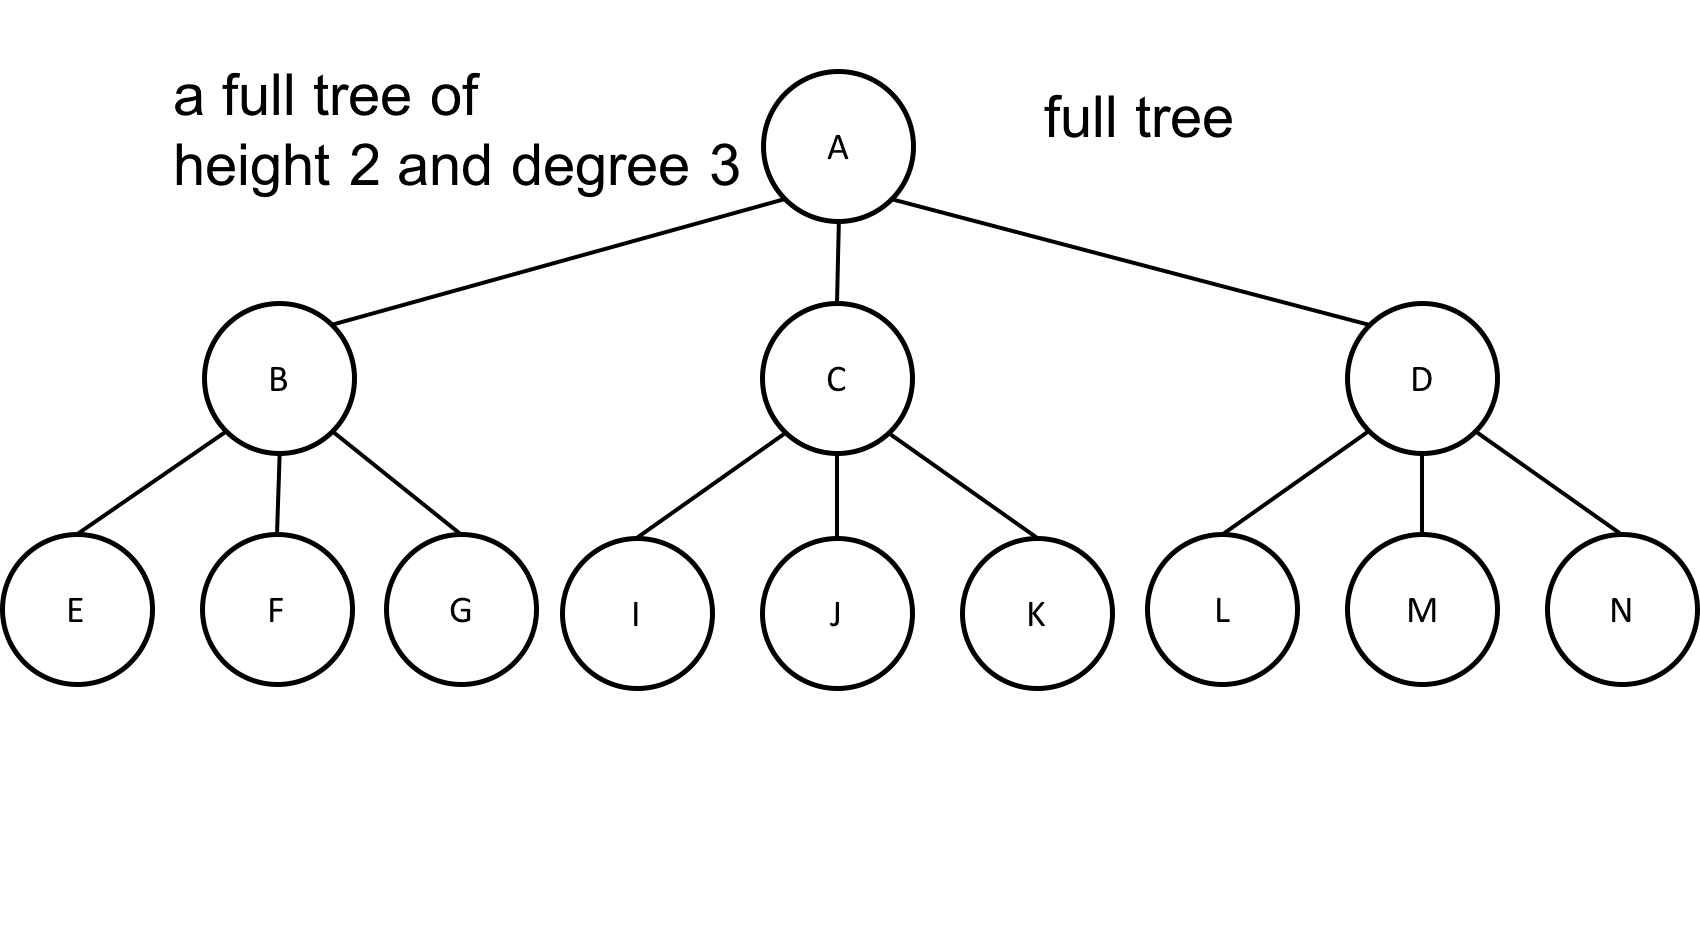
\includegraphics[height=0.3\textheight]{./figures/fig02_def_full.png}
\item[\textbf{complete tree}] All levels are full except for the deepest level, which is partially filled from the left\\
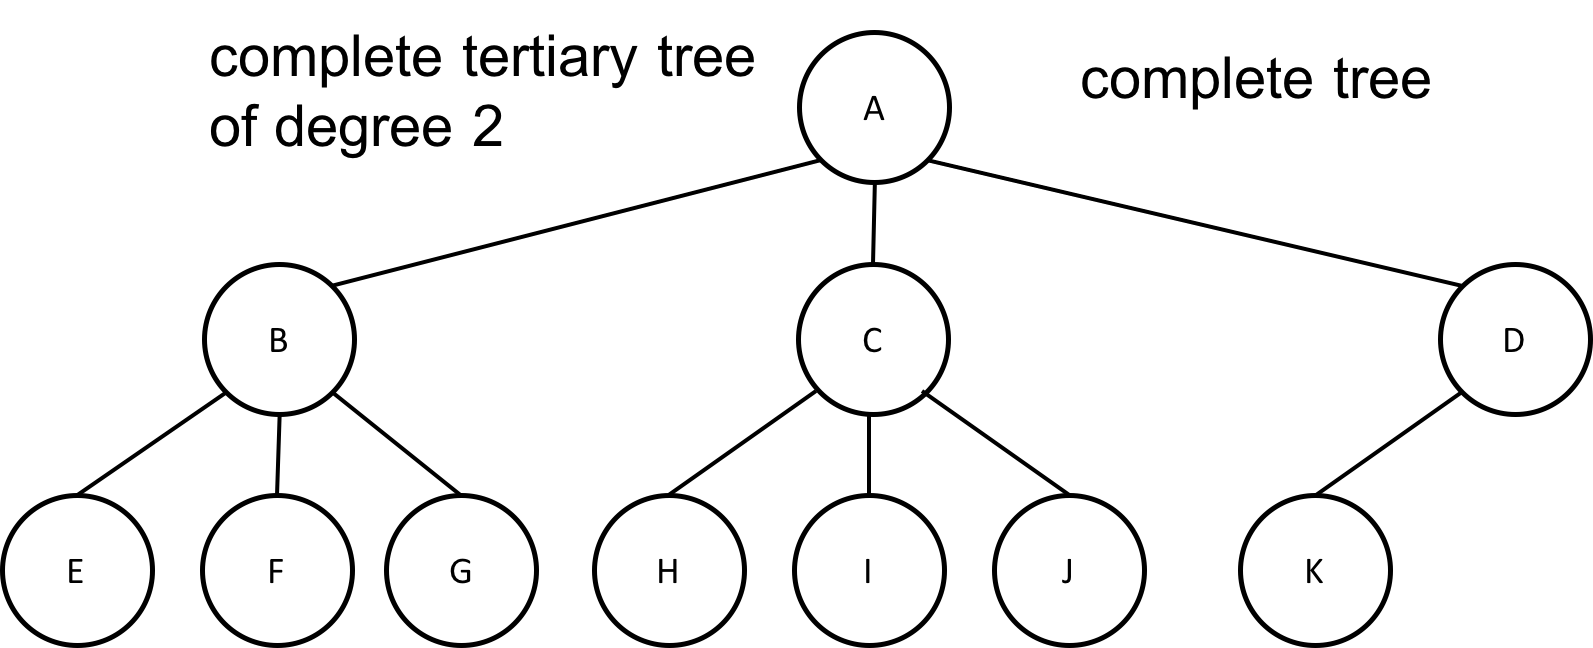
\includegraphics[height=0.3\textheight]{./figures/fig02_def_complete.png}
  \end{description}
\end{frame}

\section{Tree Representation}

\begin{frame}[t]
  \frametitle{Tree Data Structure}
Two types of representation of tree
  \begin{enumerate}
  \item List representation
  \item left child - right sibling representation
  \end{enumerate}
\end{frame}


\begin{frame}[t]
  \frametitle{List Representation}
Two types of nodes
  \begin{enumerate}
  \item Node with data
  \item Node with the reference
  \end{enumerate}

The information in the root node comes first and it is followed by a list of the subtrees of that node
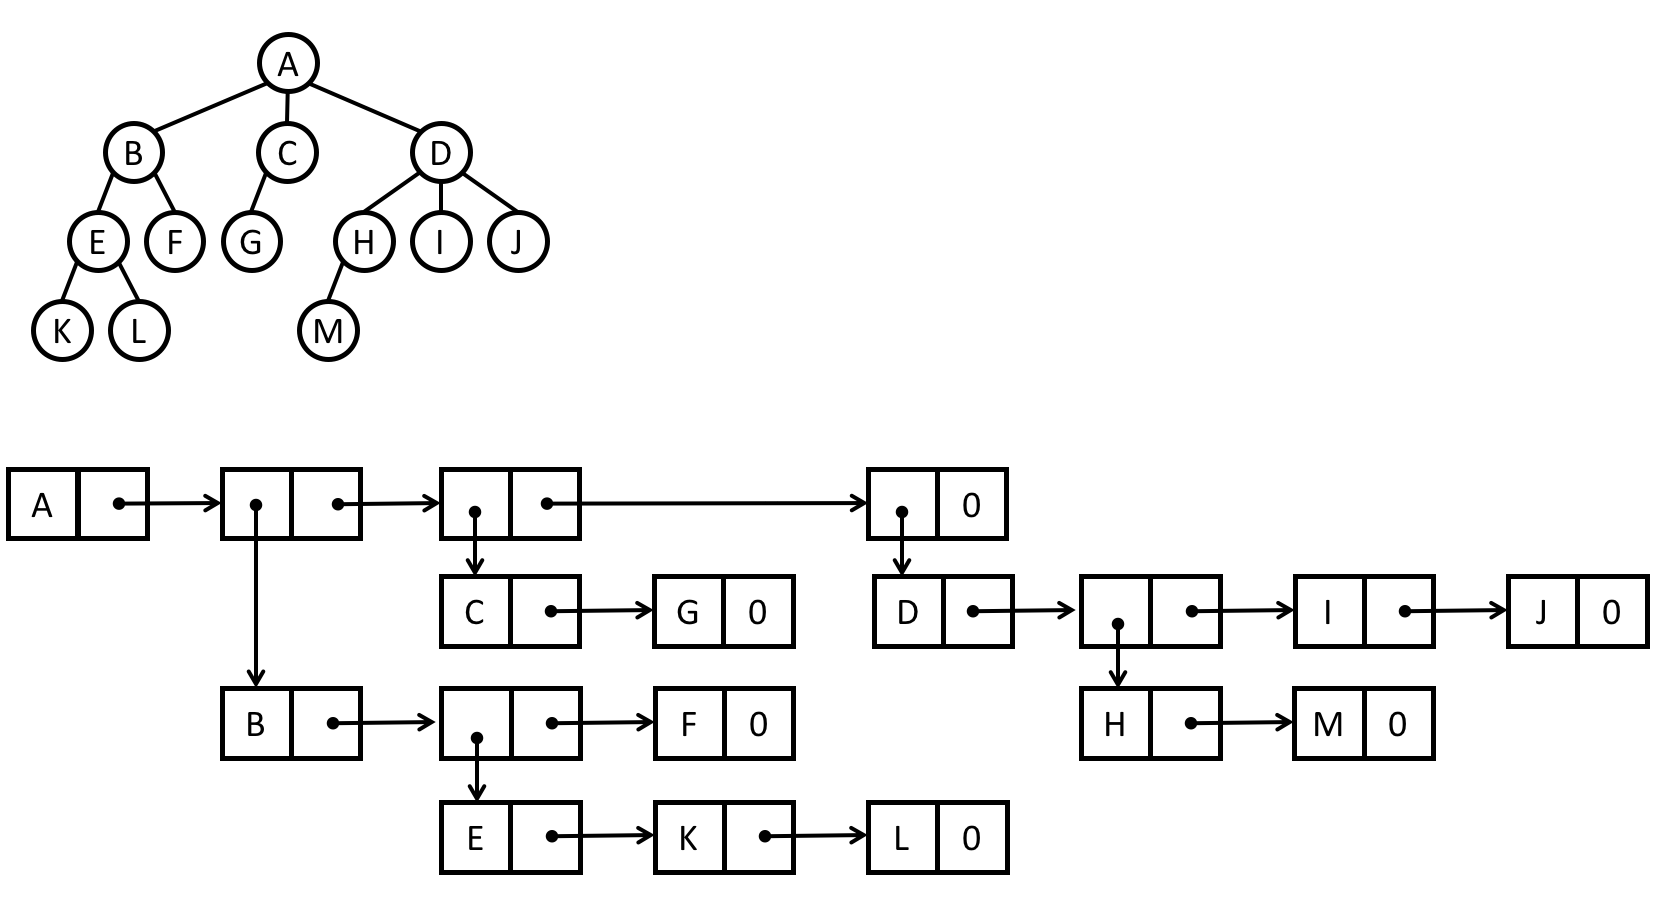
\includegraphics[height=0.6\textheight]{figures/fig03_list_rep.png}
\end{frame}


\begin{frame}[t]
  \frametitle{Left-child Right-Sibling Representation}
nodes of a fixed size
\begin{itemize}
\item easier to work
\item two link / pointer fields and a data field per node
  \begin{itemize}
  \item left reference field stores the address of the left child
  \item right reference field stores the address of the right sibling node
  \end{itemize}
\end{itemize}
\begin{center}
  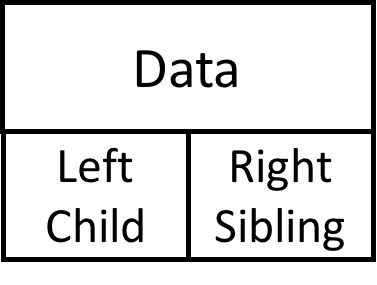
\includegraphics[width=0.2\textwidth]{figures/fig03_left-right.png}
\end{center}

\end{frame}



\begin{frame}[t]
  \frametitle{Left-child Right-sibling Representation}
  \begin{center}
    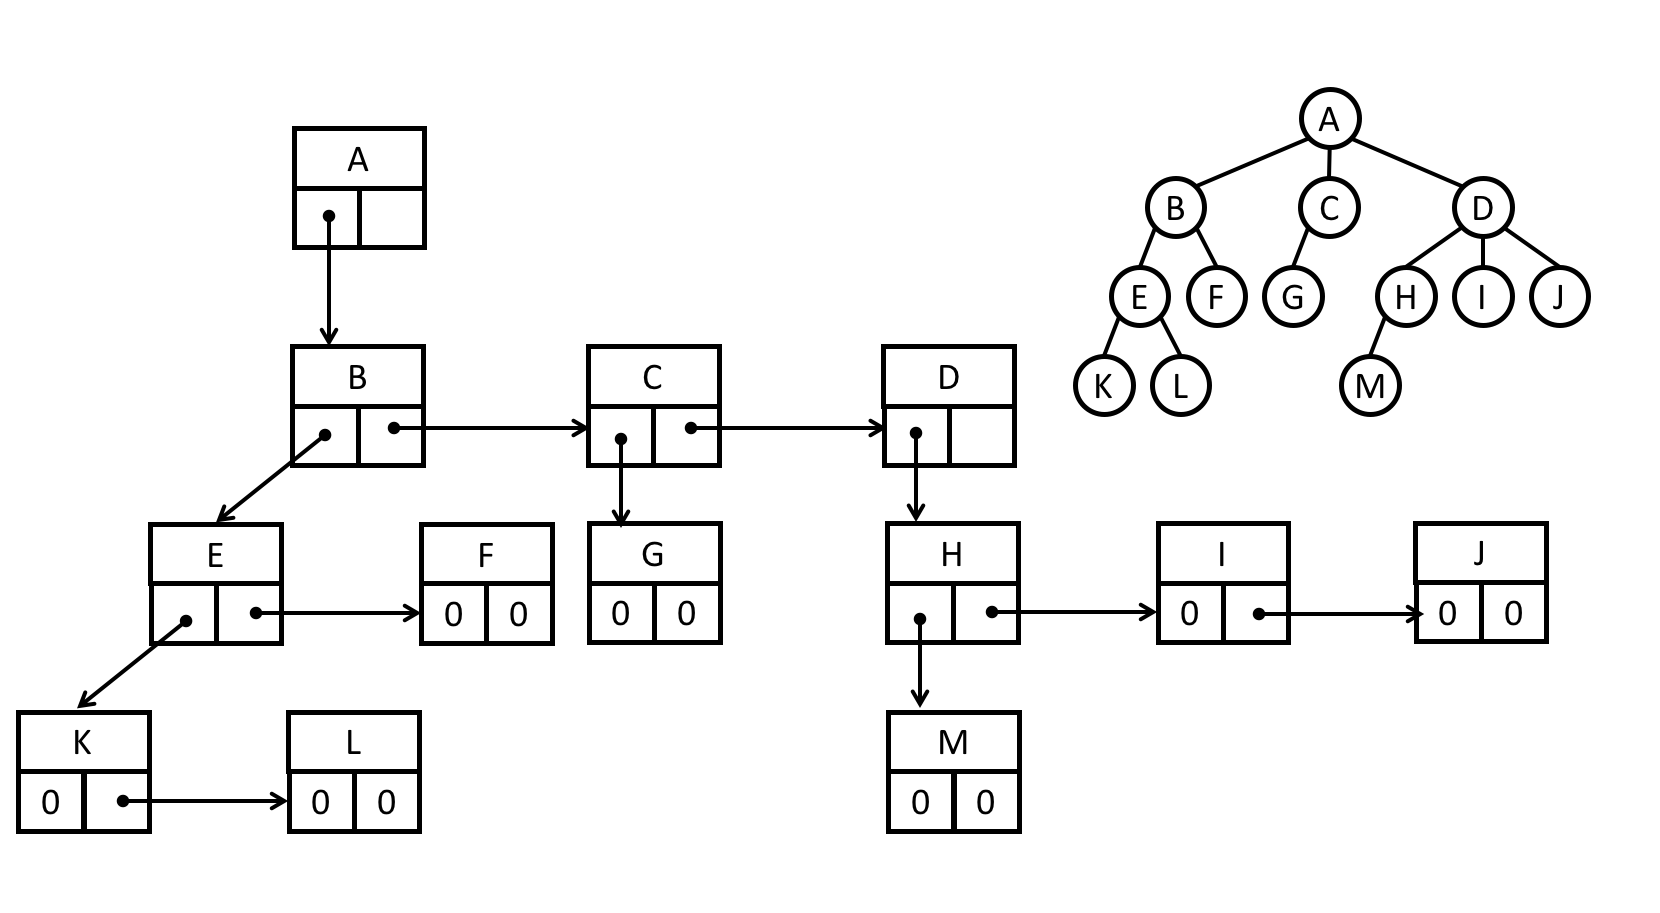
\includegraphics[width=0.9\textwidth]{figures/fig03_child-sibling.png}
  \end{center}

\end{frame}


\begin{frame}[t]
  \frametitle{Representation of trees}
Changing a representation of a tree as a degree two tree
\begin{itemize}
\item simply rotate the left-child right-sibling tree clockwise by 45 degrees
\end{itemize}

A tree with degree 2 (two children, left and right child) is called a binary tree

  \begin{center}
    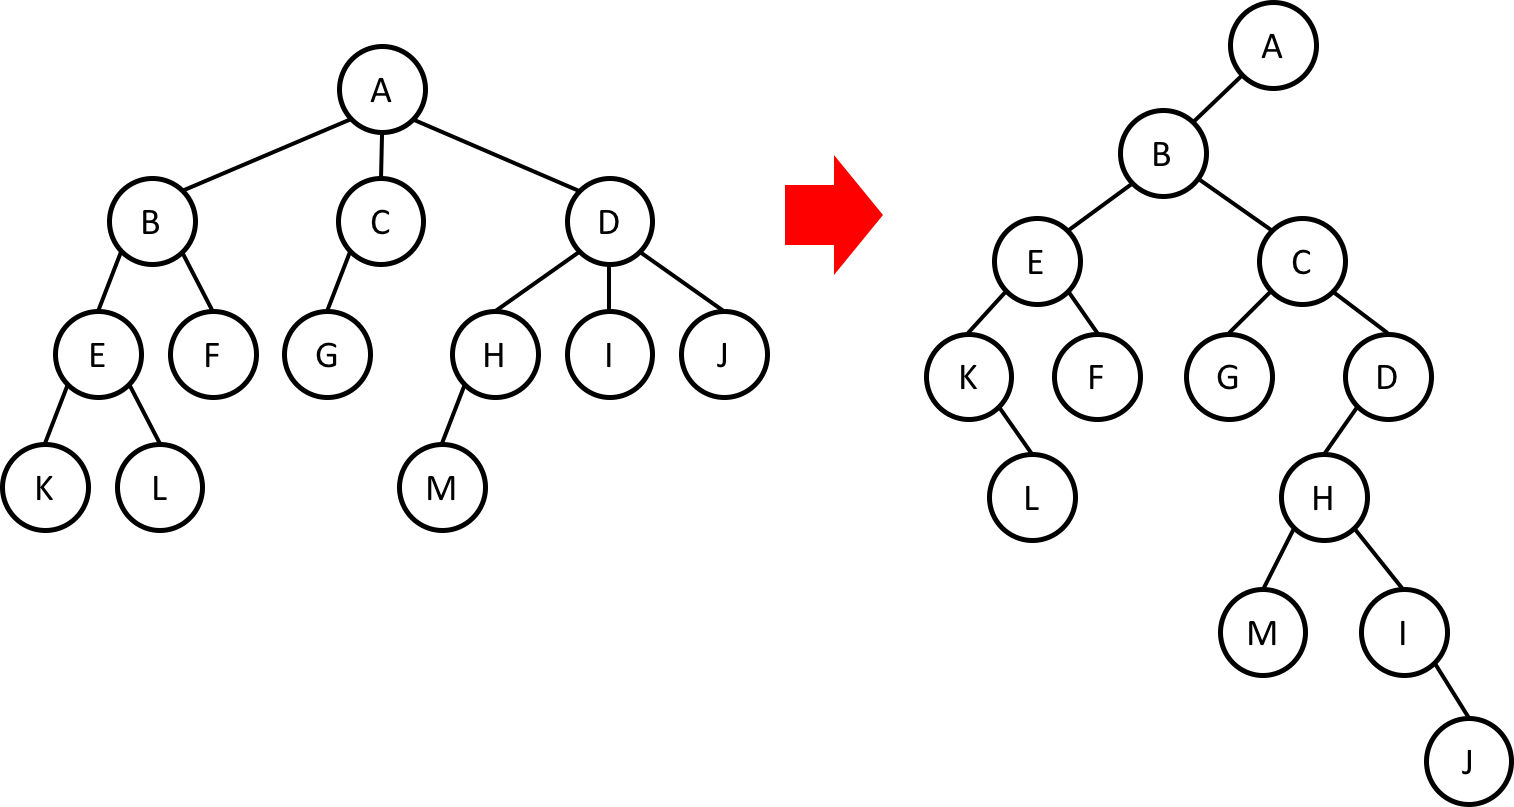
\includegraphics[width=0.8\textwidth]{figures/fig04_bin.png}
  \end{center}

\end{frame}

\section{Binary Tree}


\begin{frame}[t]
  \frametitle{Definition}
A binary Tree is a finite set of nodes such that
\begin{enumerate}
\item empty or
\item consists of root note and two disjoint binary trees, called left subtree and right subtree
\end{enumerate}


\begin{figure}
  \centering
  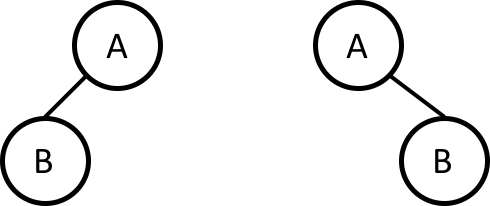
\includegraphics[width=0.3\textwidth]{figures/fig05_binary_def.png}
\caption{two different types of binary tree}
\end{figure}
\end{frame}


\begin{frame}[t]
  \frametitle{Properties}
Difference between a binary tree and a tree
\begin{itemize}
\item may have empty node
\item the order of subtree are important
\item a  binary tree is not a subset of a tree
\item maximum number of nodes in a Binary Tree is $2^k -1$ where k is
  depth of the tree
\item relationship between the number of leaf nodes ($n0$) and the
  number of nodes with degree 2 ($n2$) $ n0 =n2 +1$
\end{itemize}

\end{frame}


\begin{frame}[t, allowframebreaks]
  \frametitle{Special Types of Binary Trees}
  \begin{itemize}
  \item skewed binary tree \\
     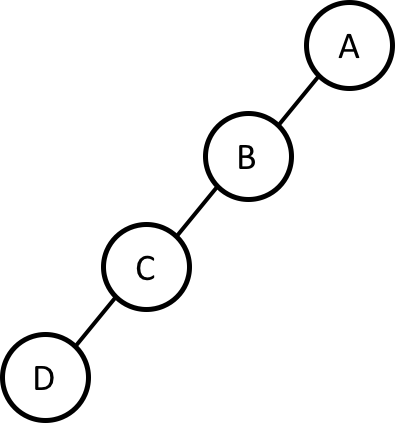
\includegraphics[height=0.3\textheight]{figures/fig06_skewed.png}
\newpage
~\bigskip
  \item full binary tree (of depth k) 
    \begin{description}
    \item[\textbf{full (or proper or strictly binary tree}] every node has either two or zero number of children \\
 
        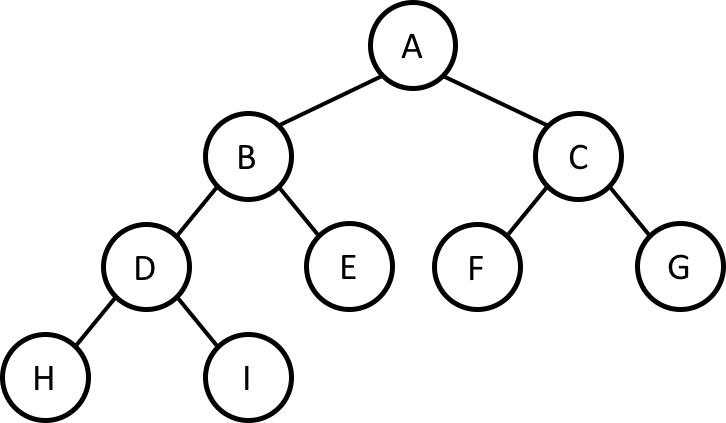
\includegraphics[height=0.3\textheight]{figures/fig06_full.png}
 
\newpage
~\bigskip
    \end{description}
  \item complete binary tree 
    \begin{description}
    \item[\textbf{complete (or perfect) binary tree}] A binary tree in which every internal node has exactly two children and all leaf nodes are at same level
a binary tree with n nodes that
      correspond to the nodes numbered from 1 to n in the full binary
      tree of depth k\\
        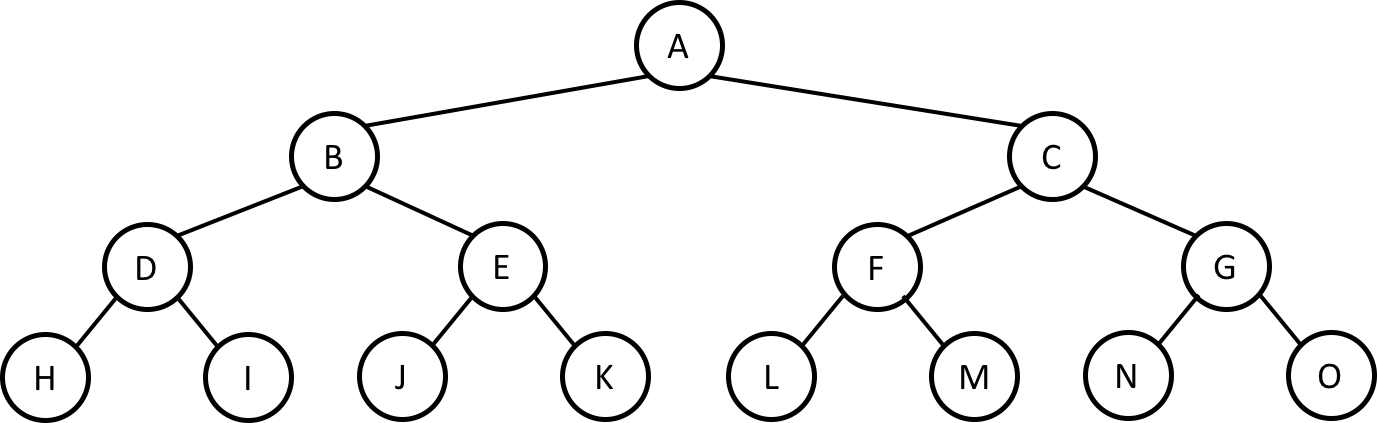
\includegraphics[height=0.3\textheight]{figures/fig06_complete.png}


    \end{description}

  \end{itemize}

\end{frame}


\begin{frame}[t]
  \frametitle{Binary Tree Representation}
There are two methods to represent the binary tree
\begin{enumerate}
\item Array Representation
\item Linked List Representation
\end{enumerate}
\end{frame}


\begin{frame}[t]
  \frametitle{Array Representation}
  \begin{itemize}
  \item sequential representations
  \item determine the locations of the parent, left child, and right
    child of any node i in the binary tree
    \begin{enumerate}
    \item parent (i) is at $\lfloor i/2 \rfloor$ if $i \neq 1$, if $i = 1$, no parent
    \item left\_child (i) is at $2 \cdot i$ if $2i \leq n$
    \item right\_child (i) is at $2 \cdot i + 1$ if $2 \cdot i+1 \leq n$

    \end{enumerate}
        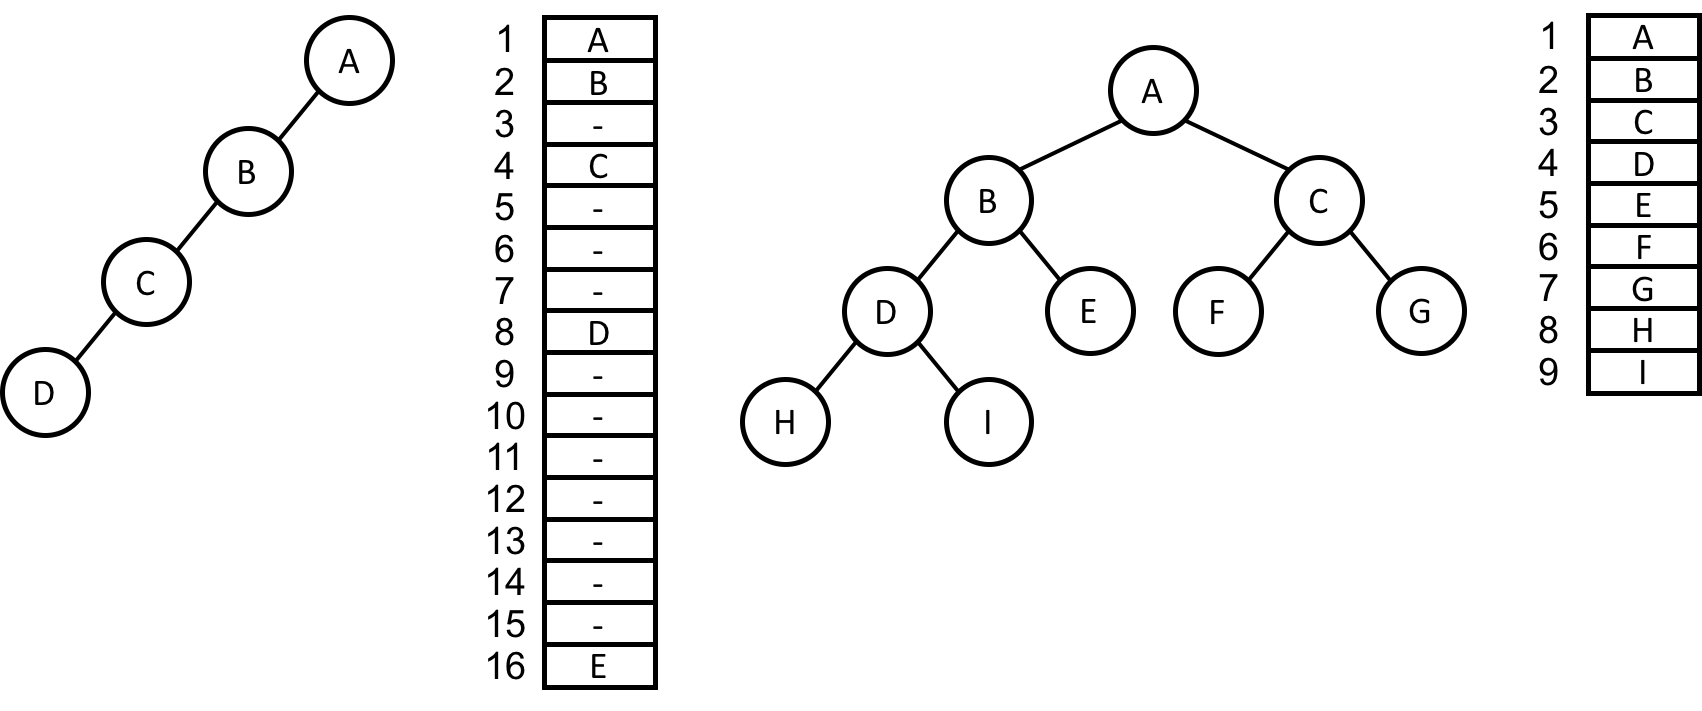
\includegraphics[height=0.5\textheight]{figures/fig07_skewed_array.png}
  \end{itemize}


\end{frame}


\begin{frame}[t]
  \frametitle{The Problem of Array Representation of Tree}
  \begin{itemize}
  \item inefficient storage utilization \\
        $S(n) = 2 -1$ where k is  depth of binary tree\\
         ideal for complete binary trees
  \item hard to insert/delete
  \end{itemize}

\end{frame}


\begin{frame}[t, fragile]
  \frametitle{Linked List representation}
Representing tree with linked list
\begin{itemize}
\item each node has three fields
  \begin{enumerate}
  \item left\_child
  \item data
  \item right\_child
  \end{enumerate}
\end{itemize}

\begin{lstlisting}
typedef struct node {
    int data;
    node left_child, right_child;
};
\end{lstlisting}
\begin{center}
        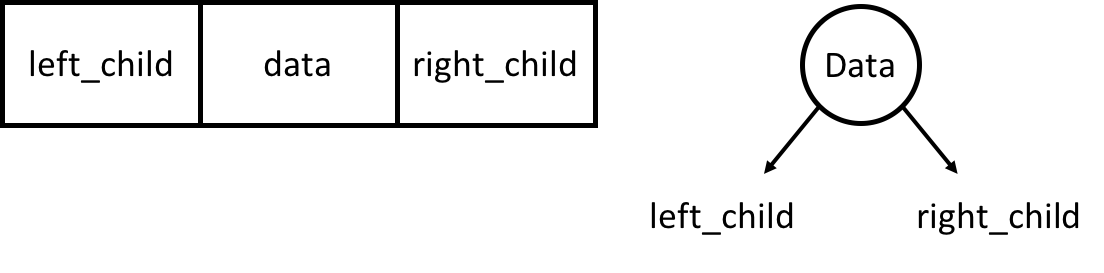
\includegraphics[height=0.2\textheight]{figures/fig08_linked_list.png}
\end{center}
\end{frame}


\begin{frame}[t]
  \frametitle{example}
Skewed

  \begin{center}
\vspace{-1em}
    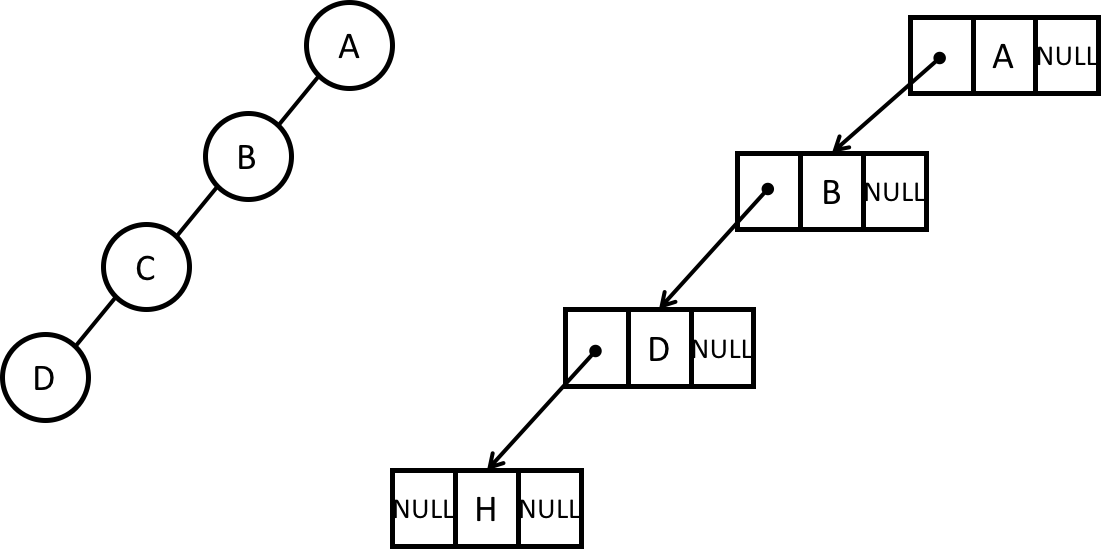
\includegraphics[height=0.3\textheight]{figures/fig08_linked_list_skewed.png}
  \end{center}

complete 
  \begin{center}
\vspace{-1em}
    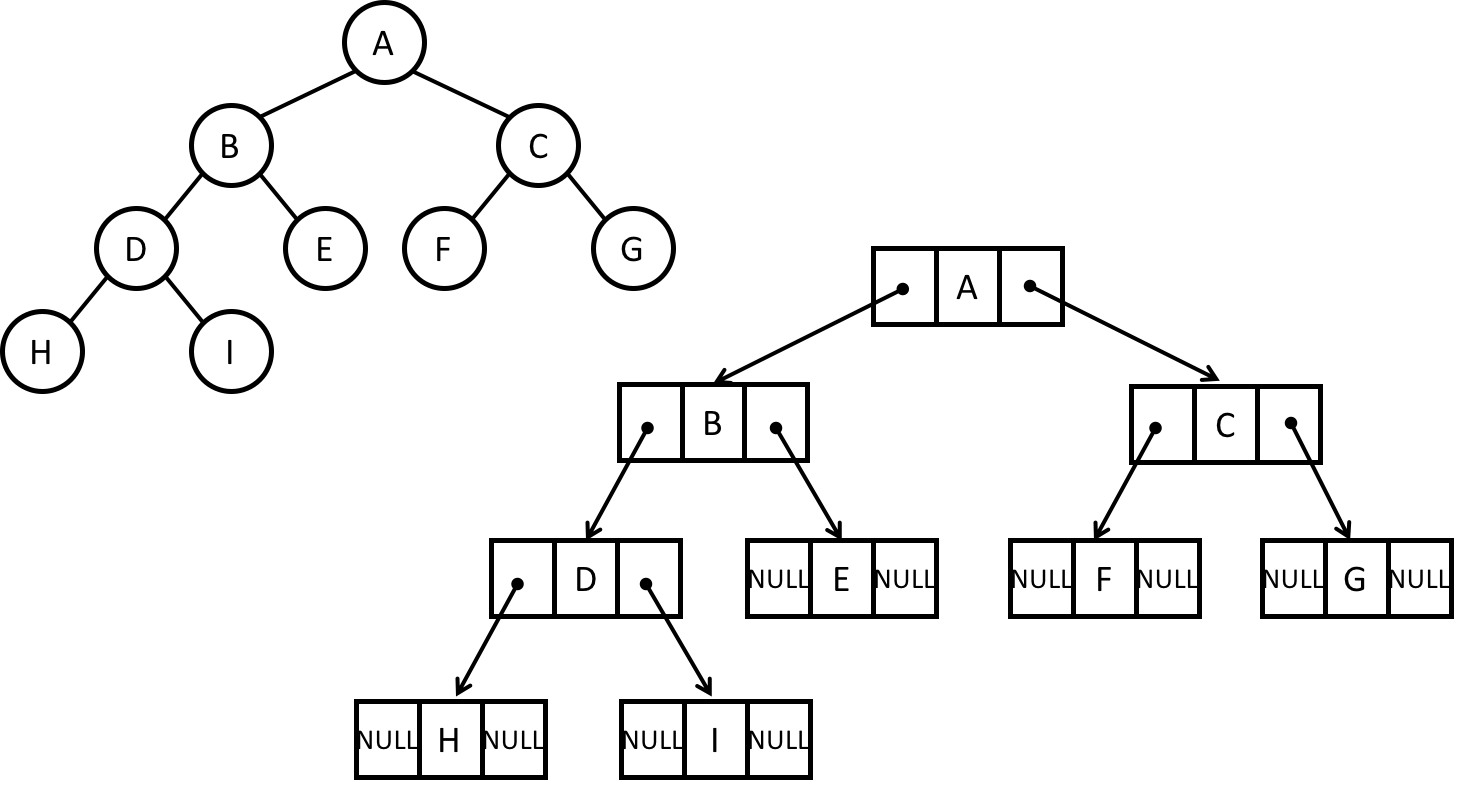
\includegraphics[height=0.4\textheight]{figures/fig08_linked_list_complete.png}
  \end{center}

\end{frame}


\begin{frame}[t]
  \frametitle{Linked List Representation cont'd}
leaf node's link field contains NULL pointer

  \begin{center}
\vspace{-1em}
    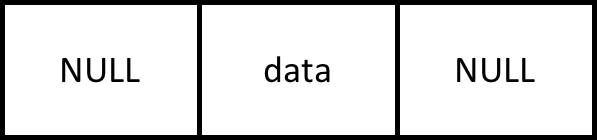
\includegraphics[width=0.3\textwidth]{figures/fig08_linked_list2.png}
  \end{center}

Add a fourth field, called parent, to know the parent of a random nodes
  \begin{center}
\vspace{-1em}
    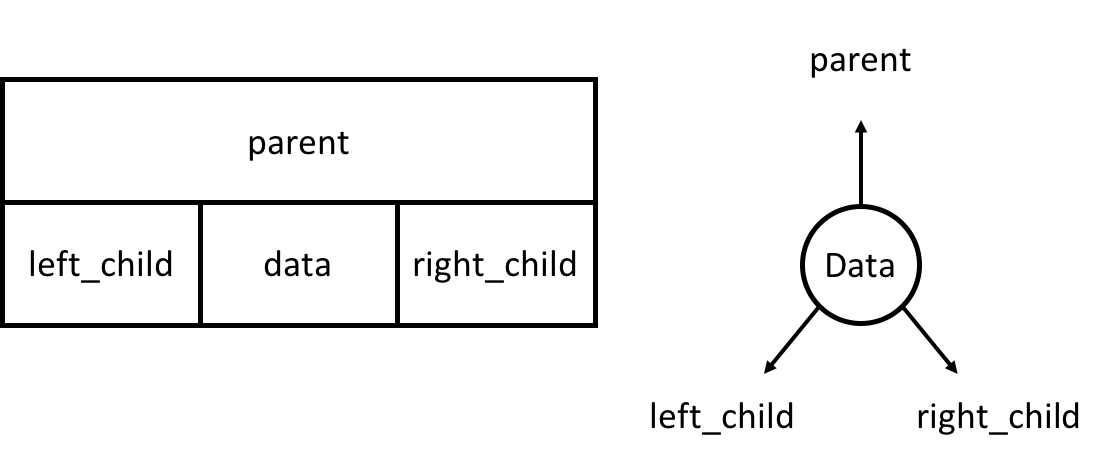
\includegraphics[width=0.5\textwidth]{figures/fig08_linked_list1.png}
  \end{center}

\end{frame}



\begin{frame}[t]
  \frametitle{Tree Representation}
  \begin{itemize}
  \item each node in a tree has a variable sized nodes
  \item hard to represent it by using array
  \item use linked list to represent a tree needs k link fields per node where k is degree of tree
  \item There are two types of links
    \begin{itemize}
    \item non-null links
    \item null links
    \end{itemize}
  \item number of non-null links are $n-1$
  \item number of null links are $n \cdot k - (n-1)$
  \end{itemize}
\end{frame}


\begin{frame}[t]
  \frametitle{Converting a tree into a binary Tree}
  \begin{enumerate}
  \item (parent, $child_1$, $child_2$, $\ldots$, $child_x$) $\rightarrow$ 
        (parent, leftmost-child, next-right-sibling) $\rightarrow$  
        left-child right-sibling representation
   \item simply rotate the left-child right-sibling tree clockwise by 45 degrees
     \begin{itemize}
     \item right field of root node always have null link
     \item null links: approximately 50$\%$
     \item depth increased
     \end{itemize}

  \end{enumerate}
\end{frame}


\begin{frame}[t]
  \frametitle{Converting a tree into a binary Tree}
  \begin{center}
    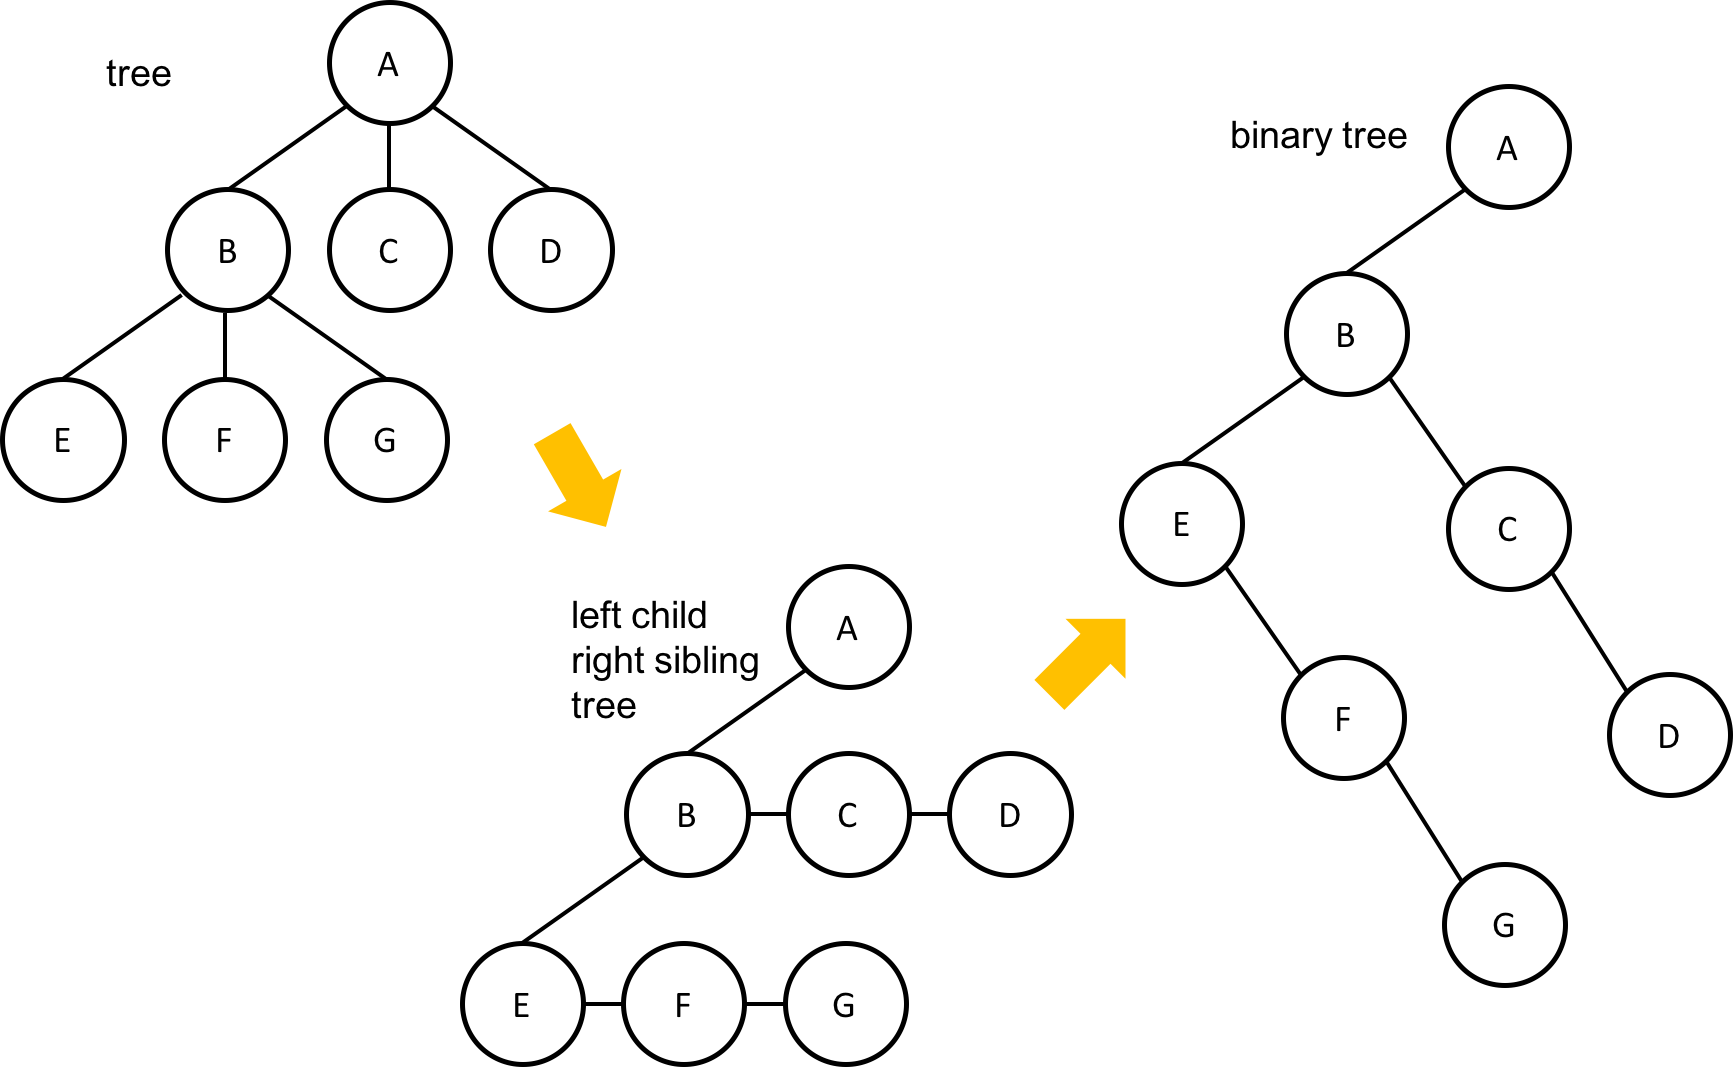
\includegraphics[width=0.8\textwidth]{figures/fig09_conversion.png}
  \end{center}

\end{frame}


\section{Binary Tree Traversal and Other Operations}
\begin{frame}[t]
  \frametitle{Binary Tree Traversals}
visit each node in the tree exactly once
\begin{itemize}
\item produce a linear order for the information in a tree
\item what order?
  \begin{itemize}
  \item inorder: LVR (Left Visit Right)
  \item preorder: VLR (Visit Left Right)
  \item postorder: LRV (Left Right Visit)
  \end{itemize}
\end{itemize}

\end{frame}


\begin{frame}[t]
  \frametitle{Binary Tree Traversals}
$A/B*C*D+E$ (infix form)
  \begin{center}
    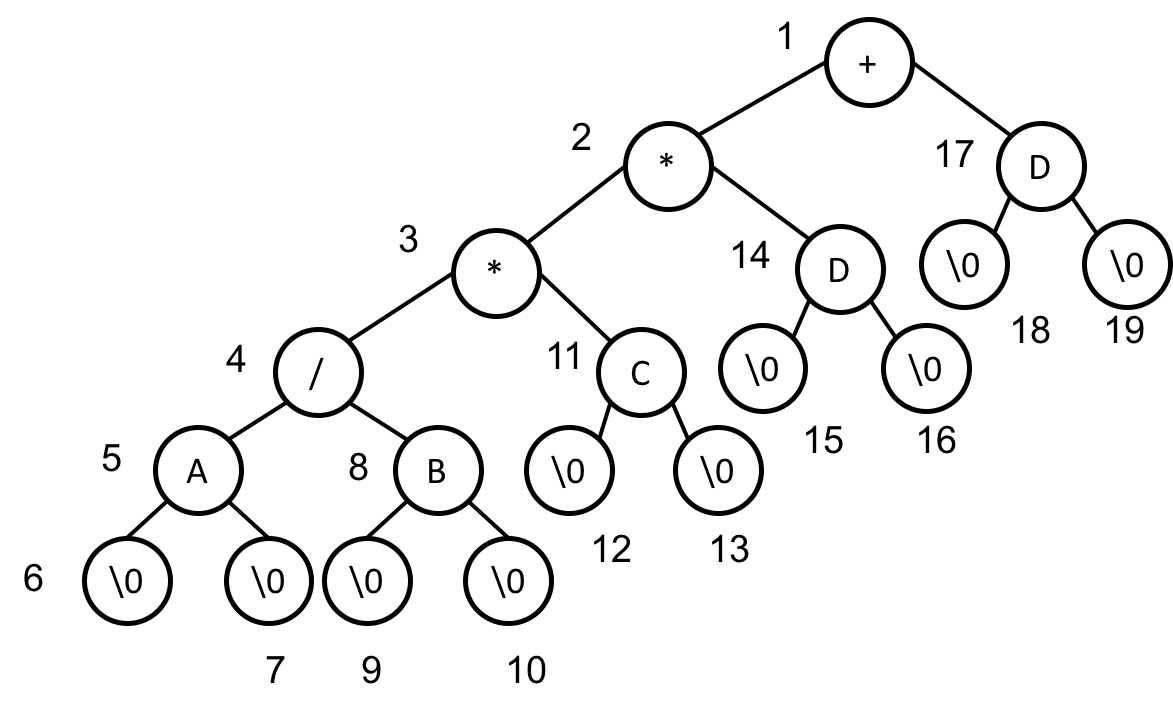
\includegraphics[width=0.8\textwidth]{figures/fig10_infix.png}
  \end{center}

\end{frame}


\begin{frame}[t, fragile]
  \frametitle{Binary Tree Traversals}
Inorder Traversal

\begin{lstlisting}
void inorder(tree_ptr ptr) { 
    if(ptr) {
        inorder(ptr->left_child); 
        printf("%d",ptr->data); 
        inorder(ptr->right_child);
    } 
}  
\end{lstlisting}
inorder is invoked 19 times for the complete traversal: 19 nodes

output: $A/B*C*D+E$
\begin{itemize}
\item  corresponds to the infix form
\end{itemize}

\end{frame}

\begin{frame}[t]
  \frametitle{Binary Tree Traversal}
  \begin{tabular}{p{4em} p{4em} c || p{4em} p{4em} c}
call of inorder & value in root & action & call of inorder & value in root & action \\
1	&	+	&		&	11	&	C	&		\\
2	&	*	&		&	12	&	NULL	&		\\
3	&	*	&		&	11	&	C	&	printf	\\
4	&	/	&		&	13	&	NULL	&		\\
5	&	A	&		&	2	&	*	&	printf	\\
6	&	NULL	&		&	14	&	D	&		\\
5	&	A	&	printf	&	15	&	NULL	&		\\
7	&	NULL	&		&	14	&	D	&	printf	\\
4	&	/	&	printf	&	16	&	NULL	&		\\
8	&	B	&		&	1	&	+	&	printf	\\
9	&	NULL	&		&	17	&	E	&		\\
8	&	B	&	printf	&	18	&	NULL	&		\\
10	&	NULL	&		&	17	&	E	&	printf	\\
3	&	*	&	printf	&	19	&	NULL	&		\\    
  \end{tabular}
\end{frame}


\begin{frame}[t, fragile]
  \frametitle{Preorder Traversal}

\begin{lstlisting}
void preorder(tree_ptr ptr) { 
    if(ptr) {
        printf("%d",ptr->data); 
        preorder(ptr->left_child); 
        preorder(ptr->right_child);
    } 
}  
\end{lstlisting}

output in the order $+**/ABCDE$

\end{frame}


\begin{frame}[t, fragile]
  \frametitle{Postorder Traversal}
\begin{lstlisting}
void postorder(tree_ptr ptr) { 
    if(ptr) {
        postorder(ptr->left_child); 
        postorder(ptr->right_child);
        printf("%d",ptr->data); 
    } 
}  
\end{lstlisting}

output in the order $AB/C*D*E+$

\end{frame}


\begin{frame}[t]
  \frametitle{Iterative Inorder Traversal}
Recursion
\begin{itemize}
\item call itself directly or indirectly
\item simple, compact expression: good
readability
\item don’t need to know implementation
details
\item much storage: multiple activations
exist internally
\item  slow execution speed
\item  application: factorial, Fibonacci
number, tree traversal, binary search, tower of Hanoi, quick sort, LISP structure
\end{itemize}
\end{frame}


\begin{frame}[t, fragile]
  \frametitle{Iterative Inorder traversal}
  \begin{lstlisting}
void iter_inorder(tree_ptr node) { 
    int top = -1;
    tree_ptr stack[MAX_STACK_SIZE]; 
    while (1) {
        while (node) {
            push(&top, node);
            node = node->left_child;
        }
        node = pop(&top);
        if (!node) break; 
        printf("%d", node->data); 
        node = node->right_child;
    } 
}    
  \end{lstlisting}
\end{frame}


\begin{frame}[t]
  \frametitle{Iterative Inorder Traversal}
every node of the tree is placed on and removed from the stack exactly once

\begin{itemize}
\item time complexity: O(n) where n is the number of nodes in the tree
\item space complexity: stack size O(n) where n is worst case depth of the
  tree (case of skewed binary tree)
\end{itemize}

\end{frame}


\begin{frame}[t]
  \frametitle{Level Order Traversal}
Traversal by using queue (FIFO)

  \begin{center}
    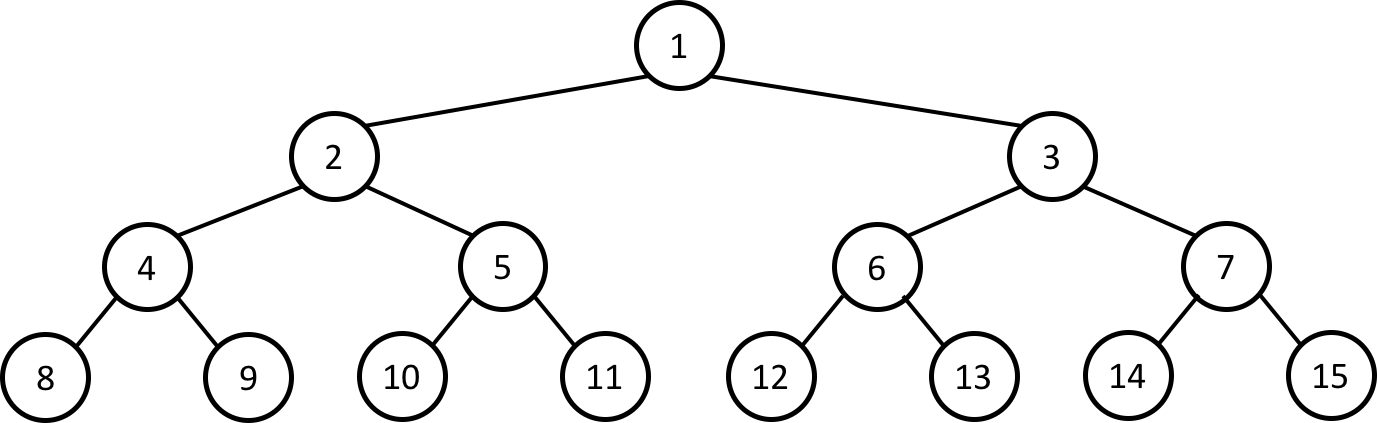
\includegraphics[width=0.8\textwidth]{figures/fig11_level_order.png}
  \end{center}

Output in the order: 1, 2, 3, 4, $\ldots$, 14, 15
\end{frame}


\begin{frame}[t, fragile]
  \frametitle{Level Order Traversal}
  \begin{lstlisting}
void level_order(tree_ptr ptr) { 
    int front = rear = 0;
    tree_ptr queue[MAX_QUEUE_SIZE]; 

    if (!ptr) return; 

    addq(front,&rear,ptr);

    while (1) {
        ptr = deleteq(&front, rear); 

        if (ptr) {
            printf("%d", ptr->data); 
            if (ptr->left_child)
                addq(front,&rear,ptr->left_child); 
            if (ptr->right_child)
                addq(front,&rear,ptr->right_child); 
            else break;
        }
    } 
}    
  \end{lstlisting}
\end{frame}


\begin{frame}[t, fragile]
  \frametitle{Copying Binary Tree}
Modified version of postorder
\begin{lstlisting}
tree_ptr copy(tree_ptr original) {
    tree_ptr temp; 
    if (original) {
        temp = (tree_ptr)malloc(sizeof(node)); 

        if (IS_FULL(temp)) exit(1); 
            temp->left_child = copy(original->left_child); 
            temp->right_child = copy(original->right_child); 
            temp->data = original->data; 
            return temp;
         }
    return NULL; 
}  
\end{lstlisting}
\end{frame}


\begin{frame}[t, fragile]
  \frametitle{Testing for equality of binary trees}
Modified version of preorder
\begin{lstlisting}
int equal(tree_ptr first, tree_ptr second) {
return ((!first && !second) || 
       (first && second 
       && (first->data == second->data) 
       && equal(first->left_child,
                second->left_child) 
       && equal(first->right_child,
                second->right_child));
}
\end{lstlisting}
\end{frame}

\section{Heaps}
\begin{frame}[t]
  \frametitle{Heaps: Definition}
  \begin{description}
  \item[\textbf{MAX (or MIN) Tree}] a tree in which the key value in each node is no smaller (larger) than the key value in its children (if any)
  \item [\textbf{MAX (or MIN) Heap}] a complete binary tree that is also a max (or min) tree
  \end{description}
  \begin{itemize}
  \item the root of a max (or min) tree contains the largest (smallest) key in the tree
  \end{itemize}
\end{frame}


\begin{frame}[t]
  \frametitle{Representation of MAX (or MIN) heaps}
  \begin{itemize}
  \item array representation because heap is a complete binary tree

  \item simple addressing scheme for parent, left(right) child
  \end{itemize}

\end{frame}


\begin{frame}[t, fragile]
  \frametitle{Heap Structure}
  \begin{lstlisting}
#define MAX_ELEMENTS 200
#define HEAP_FULL(n) (n == MAX_ELEMENTS - 1) 
#define HEAP_EMPTY(n) (!n)

typedef struct {
    int key;
    /* other field */ 
} element;

element heap[MAX_ELEMENTS]; 
int n = 0;    
  \end{lstlisting}
\end{frame}


\begin{frame}[t]
  \frametitle{Sample Max Heaps}
  \begin{center}
    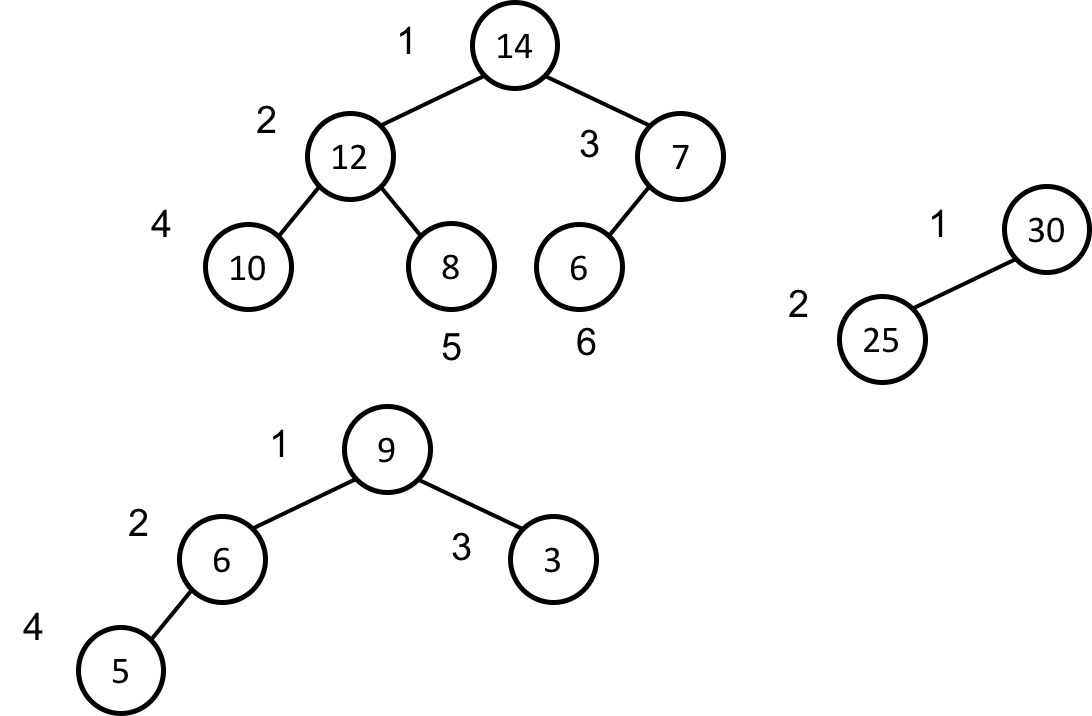
\includegraphics[width=0.8\textwidth]{figures/fig12_sample_heap.png}
  \end{center}

\end{frame}


\begin{frame}[t]
  \frametitle{Sample Min Heaps}
  \begin{center}
    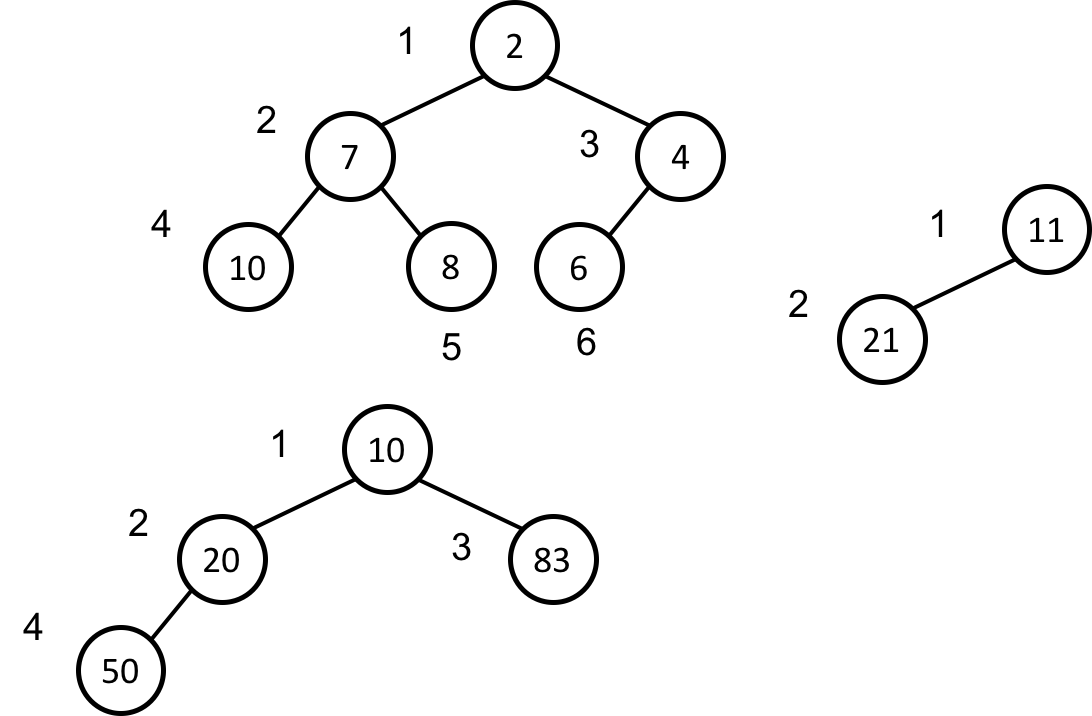
\includegraphics[width=0.8\textwidth]{figures/fig12_sample_heap1.png}
  \end{center}

\end{frame}


\begin{frame}[t]
  \frametitle{Priority Queues}
  \begin{description}
  \item [\textbf{deletion}] deletes the element with the highest(or
    the lowest) priority
  \item [\textbf{insertion}] insert an element with arbitrary priority
    into a priority queue at any time
  \end{description}
Ex. Job scheduling of OS
\end{frame}


\begin{frame}[t]
  \frametitle{Priority Queues}
We use a max (or Min) Heap to implement the Priority Queues

Possible priority queue representations

\begin{tabular}{l c c}
  Representation & insertion & deletion \\ \hline \hline
unordered array & O(1) & O(n) \\
unordered linked list & O(1) & O(n) \\
sorted array & O(n) & O(1) \\
sorted linked list & O(n) & O(1) \\
max heap & O($log_2n$) &  O($log_2n$) \\
\end{tabular}
\end{frame}


\begin{frame}[t]
  \frametitle{Insertion into a max heap}
Need to go from a node to its parent
\begin{itemize}
\item linked representation add a parent field to each node
  \item array representation a heap is a complete binary tree simple
    addressing scheme
\end{itemize}
\end{frame}


\begin{frame}[t]
  \frametitle{Insertion into a max heap}
  \begin{tabular}{p{0.44\textwidth} p{0.44\textwidth}}
Heap before Insertion

    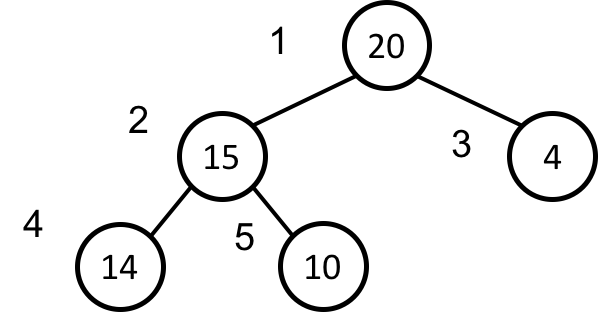
\includegraphics[width=0.4\textwidth]{./figures/fig13_heap_insert.png}
&    
  Initial location of new node

    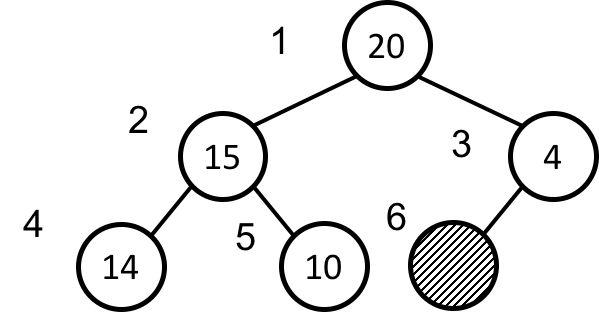
\includegraphics[width=0.4\textwidth]{./figures/fig13_heap_insert1.png}
\pause \\
~& ~\\
Insert 5 into heap

    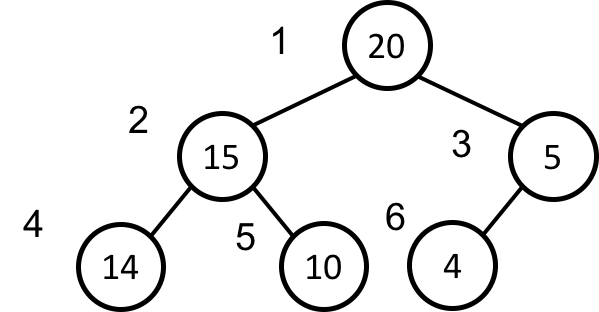
\includegraphics[width=0.4\textwidth]{./figures/fig13_heap_insert2.png}
&
Insert 35 into heap

    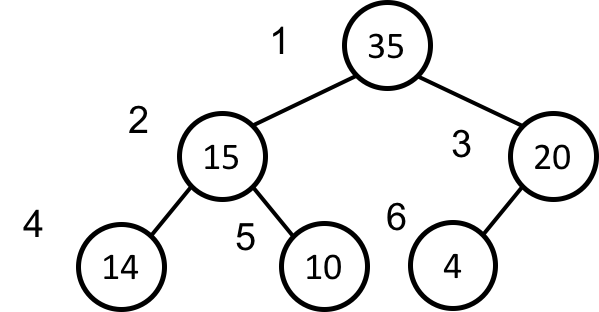
\includegraphics[width=0.4\textwidth]{./figures/fig13_heap_insert3.png}
\\
  \end{tabular}
\end{frame}


\begin{frame}[t]
  \frametitle{Insertion into a max heap}
  \begin{itemize}
  \item select the initial location for the node to be inserted $\rightarrow$
    bottommost-rightmost leaf node
  \item insert a new key value adjust key
    value from leaf to root parent position: $\lfloor i/2 \rfloor$
  \item time complexity :
    $O(depth of tree) ~\rightarrow~ O(log_2n)$
  \end{itemize}
\end{frame}


\begin{frame}[t, fragile]
  \frametitle{Insertion into a max heap}
  \begin{lstlisting}
void insert_max_heap(element item, int *n) { 
    int i;
    if (HEAP_FULL(*n)) {
        fprintf(stderr,"The heap is full. \n"); 
        exit(1);
    }
    i = ++(*n);
    while ((i != 1 ) && (item.key > heap[i/2].key)) {
        heap[i] = heap[i/2]; 
        i /= 2;
    }
    heap[i] = item;     
}
  \end{lstlisting}
\end{frame}


\begin{frame}[t]
  \frametitle{Deletion from a max heap}
  \begin{itemize}
  \item always delete an element from the root of the heap
  \item restructure the tree so that it corresponds to a complete binary tree
  \item place the last node to the root and from the root compare the parent node with its children and exchanging out-of-order elements until the heap is reestablished
  \end{itemize}
\end{frame}


\begin{frame}[t]
  \frametitle{Deletion from a max heap}
  \begin{tabular}{p{0.44\textwidth} p{0.44\textwidth}}
Heap before deletion

    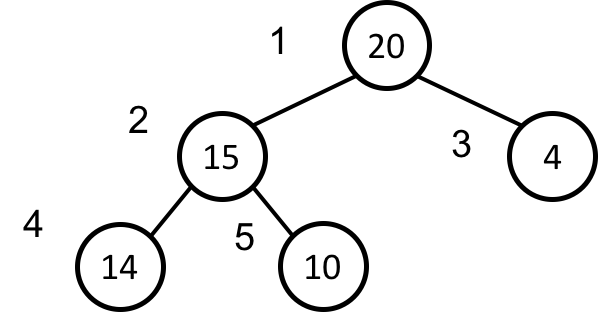
\includegraphics[height=0.3\textheight]{./figures/fig14_heap_delete.png}
&    
Heap Structure

    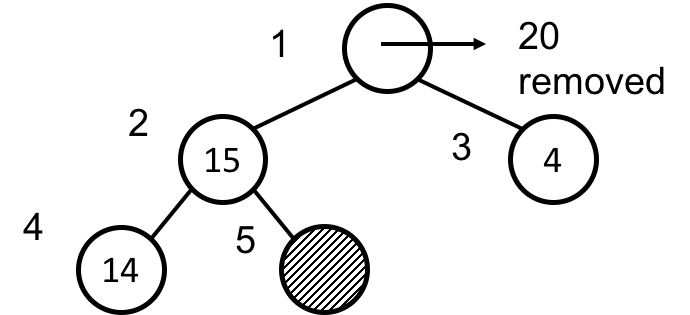
\includegraphics[height=0.3\textheight]{./figures/fig14_heap_delete1.png}
\pause \\
~& ~\\
10 inserted at the root

    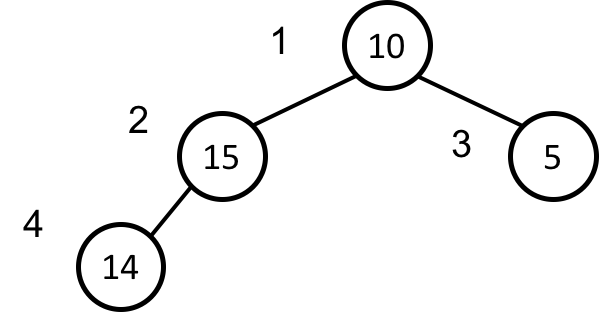
\includegraphics[height=0.3\textheight]{./figures/fig14_heap_delete2.png}
&
Final heap

    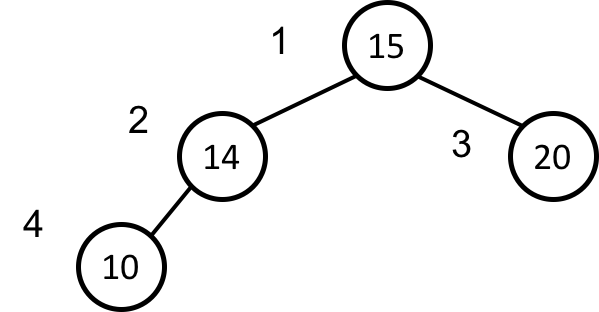
\includegraphics[height=0.3\textheight]{./figures/fig14_heap_delete3.png}
\\
  \end{tabular}
\end{frame}


\begin{frame}[t]
  \frametitle{Deletion from a max heap}
  \begin{itemize}
  \item select the removed node bottommost-rightmost leaf node
  \item place the node’s element in the root node
  \item adjust key value
    from root to leaf compare the parent node with its children and
    exchange out-of-order elements until the heap is reestablished -
  \item time complexity : $O(depth~of~ tree) \rightarrow~ O(log_2n)$
  \end{itemize}

\end{frame}


\begin{frame}[t, fragile]
  \frametitle{Deletion from a max heap}
  \begin{lstlisting}
element delete_max_heap(int *n) { 
    element item, temp;
    if (HEAP_EMPTY(*n)) {
        fprintf(stderr,"The heap is empty\n");
        exit(1); 
    }
    item = heap[1];
    temp = heap[(*n)--]; 
    parent = 1; 
    child = 2; 
    while (child <= *n) {
    /* compare left and right child’s key values */ 
        if ((child < *n) && (heap[child].key <
                             heap[child+1].key))
            child++;
        if (temp.key >= heap[child].key) break; 
        /* move to the next lower level */ 
        heap[parent] = heap[child];
        parent = child;
        child *= 2;
    }
    heap[parent] = temp; return item;
}    
  \end{lstlisting}
\end{frame}

\section{Binary Search Tree}
\begin{frame}[t]
  \frametitle{Binary Search Tree (BST)}
Binary search tree(BST) is a binary tree that is empty or each
node satisfies the following properties:
\begin{enumerate}
\item every element has a key, and no two elements have the same key
\item the keys in a nonempty left subtree must be smaller than the key
  in the root of the subtree
\item the keys in a nonempty right subtree
  must be larger than the key in the root of the subtree
\item the left and right subtrees are also BST
\end{enumerate}

\end{frame}


\begin{frame}[t]
  \frametitle{Binary Search Tree}
  \begin{tabular}{p{0.44\textwidth} p{0.44\textwidth}}
Not a BST

    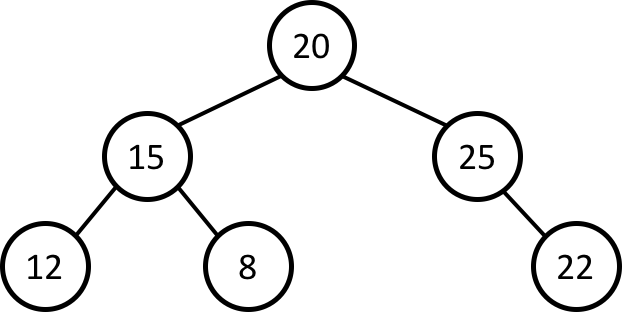
\includegraphics[height=0.3\textheight]{./figures/fig15_bst.png}
&   ~\\
~& ~\\
BST

    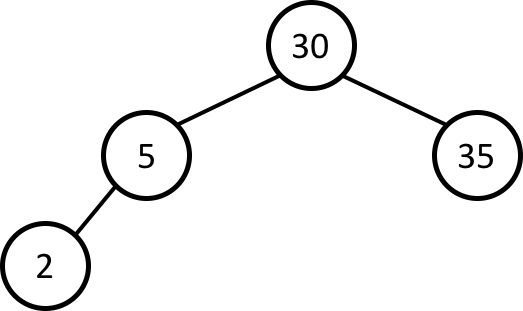
\includegraphics[height=0.3\textheight]{./figures/fig15_bst1.png}
&
BST

    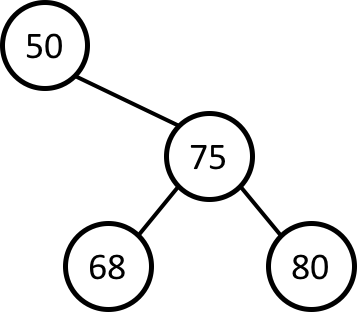
\includegraphics[height=0.3\textheight]{./figures/fig15_bst2.png}
\\
  \end{tabular}
\end{frame}


\begin{frame}[t]
  \frametitle{Operations and their Complexity}
Searching, Insertion, Deletion is bounded by $O(h)$ where h is the height of the BST

can perform these operations both
\begin{itemize}
\item by key value and\\
      e.g., delete the element with key x
\item by rank\\
      e.g., delete the fifth smallest element
\end{itemize}
\end{frame}


\begin{frame}[t, fragile]
  \frametitle{Searching a BST}

Recursive search of a BST
  \begin{lstlisting}
tree_ptr search(tree_ptr root, int key) { 
    /*  return a pointer to the node that contains
     *  key. If there is no such node, return NULL 
     */
    if (!root) return NULL;
    if (key == root->data) return root; 
    if (key < root->data) 
       return search(root->left_child, key); 
    return search(root->right_child, key);    
}
  \end{lstlisting}
\end{frame}


\begin{frame}[t, fragile]
  \frametitle{Iterative Search of a BST}
  \begin{lstlisting}
tree_ptr iter_search(tree_ptr tree, int key) {
    while (tree) {
        if (key == tree->data) return tree; 
        if (key < tree->data)
            tree = tree->left_child; 
        else
            tree = tree->right_child; 
    }
    return NULL; 
}    
  \end{lstlisting}
\end{frame}


\begin{frame}[t]
  \frametitle{Time complexity for searching}
  \begin{itemize}
  \item Average case
    \begin{itemize}
    \item $O(h)$ where h is the height of BST
    \end{itemize}
  \item Worst case
    \begin{itemize}
    \item $O(n)$ for skewed binary tree
    \end{itemize}
  \end{itemize}
\end{frame}


\begin{frame}[t, fragile]
  \frametitle{Inserting into a BST}
  \begin{lstlisting}
void insert_node(tree_ptr *node, int num) { 
    tree_ptr ptr, temp = modified_search(*node, num); 
    if (temp || !(*node)) {
        ptr = (tree_ptr)malloc(sizeof(node)); 
        if (IS_FULL(ptr)) {
            fprintf(stderr,"The memory is full\n"); 
            exit(1);
        }
        ptr->data = num;
        ptr->left_child = ptr->right_child = NULL; 
        if (*node)
            if (num < temp->data) 
                temp->left_child = ptr;
            else
                temp->right_child = ptr;
        else *node=ptr; 
    }
}
 \end{lstlisting}
\end{frame}


\begin{frame}[t, fragile]
  \frametitle{Inserting into a BST}

FIGURE-CODE??
\textbf{modified\_search} is slightly modified version of function \textbf{iter\_search}
\begin{itemize}
\item return NULL, if the tree is empty or num is present
\item otherwise, return a pointer to the last node of the tree that
  was encountered during the search
\end{itemize}

time complexity for inserting
\begin{itemize}
\item  $O(h)$, where h is the height of the tree
\end{itemize}

\end{frame}


\begin{frame}[t]
  \frametitle{Inserting into a BST}
  \begin{tabular}{p{0.44\textwidth} p{0.44\textwidth}}
Initial BST

    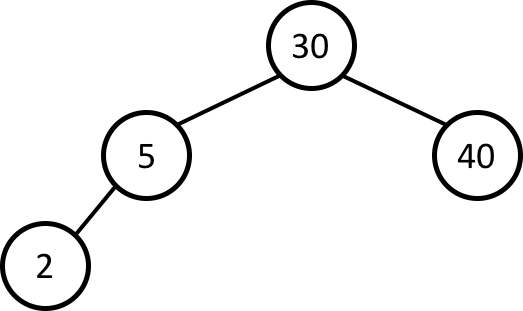
\includegraphics[height=0.3\textheight]{./figures/fig16_bst_insert.png}
&   ~\\
~& ~\\
Insert 80

    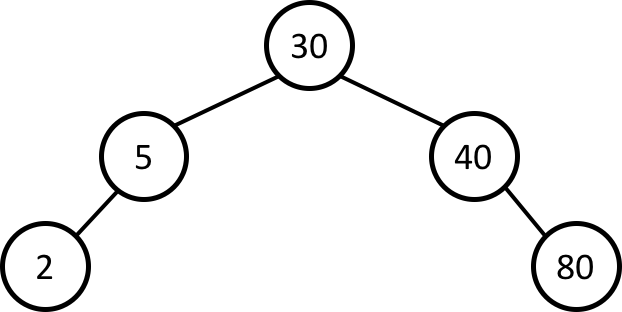
\includegraphics[height=0.3\textheight]{./figures/fig16_bst_insert1.png}
&
Insert 35

    \includegraphics[height=0.3\textheight]{./figures/fig16_bst_insert2.png}
\\
  \end{tabular}
\end{frame}


\begin{frame}[t]
  \frametitle{Deleting from  BST}
deletion of a leaf node
\begin{itemize}
\item deletion of a node with 1 child
\item deletion of a node with 2
  children
\end{itemize}

FIGURE-∗ Deleting Algorithm is discussed in Chapter 10

time complexity for deleting
\begin{itemize}
\item $O(h)$ where h is the height of the tree
\end{itemize}

\end{frame}


\begin{frame}[t]
  \frametitle{Deleting a leaf or a node with a child}
  \begin{tabular}{p{0.44\textwidth} p{0.44\textwidth}}
Initial BST

    \includegraphics[height=0.3\textheight]{./figures/fig17_bst_delete.png}
&   ~\\
~& ~\\
Delete 35 (leaf)

    \includegraphics[height=0.3\textheight]{./figures/fig17_bst_delete1.png}
&
Delete 40 (node with single child)

    \includegraphics[height=0.3\textheight]{./figures/fig17_bst_delete2.png}
\\
  \end{tabular}
\end{frame}


\begin{frame}[t]
  \frametitle{Deletion of a node with two children}
  \begin{tabular}{p{0.44\textwidth} p{0.44\textwidth}}
Tree before deletion of 60

    \includegraphics[width=0.4\textwidth]{./figures/fig17_bst_delete3.png}
&
Tree after deletion of 60

    \includegraphics[width=0.4\textwidth]{./figures/fig17_bst_delete4.png}
\\
  \end{tabular}
\end{frame}


\begin{frame}[t]
  \frametitle{Height of a BST}
the height of a BST with $n$ elements 
\begin{itemize}
\item average case: $O(log_2n)$
\item worst case: $O(n)$
  \begin{itemize}
  \item e.g., use \texttt{insert\_node} to insert the keys $1, 2, 3, \ldots, n$ into an
    initially empty BST
  \end{itemize}

\end{itemize}

\end{frame}


\begin{frame}[t]
  \frametitle{Balanced (binary) Search Tree}
  \begin{itemize}
  \item worst case height: $O(log_2n)$
  \item searching, insertion, deletion is bounded by $O(h)$ where h is
    the height of a binary tree
  \item \textit{AVL tree, 2-3 tree, red-black tree
    are all introduced in Chapter 10}
  \end{itemize}
\end{frame}


\end{document}
